\documentclass[12pt]{article}

%%%%%%%%%%%%%%%%%%%%%%%%%%%%%%%%%%%%%%%%%%%%%%%%%%%%%%%%%%%%%%%%%%%%%%%%%%%%%%%%
%                           Package preset for homework
%%%%%%%%%%%%%%%%%%%%%%%%%%%%%%%%%%%%%%%%%%%%%%%%%%%%%%%%%%%%%%%%%%%%%%%%%%%%%%%%
% Miscellaneous
\usepackage[margin=1in]{geometry}
\usepackage[utf8]{inputenc}
\usepackage{indentfirst}
\usepackage{blindtext}
\usepackage{graphicx}
\usepackage{xr-hyper}
\usepackage{hyperref}
\usepackage{enumitem}
\usepackage{color}
\usepackage{float}
% Math
\usepackage{latexsym}
\usepackage{amsfonts}
\usepackage{amssymb}
\usepackage{amsmath}
\usepackage{commath}
\usepackage{amsthm}
\usepackage{bbold}
\usepackage{bm}
% Physics
\usepackage{physics}
\usepackage{siunitx}
% Code typesetting
\usepackage{listings}
% Citation
\usepackage[authoryear]{natbib}
\usepackage{appendix}
\usepackage[capitalize]{cleveref}
% Title & name
\title{Homework}
\author{Tien Vo}
\date{\today}


%%%%%%%%%%%%%%%%%%%%%%%%%%%%%%%%%%%%%%%%%%%%%%%%%%%%%%%%%%%%%%%%%%%%%%%%%%%%%%%%
%                   User-defined commands and environments
%%%%%%%%%%%%%%%%%%%%%%%%%%%%%%%%%%%%%%%%%%%%%%%%%%%%%%%%%%%%%%%%%%%%%%%%%%%%%%%%
%%% Misc
\sisetup{load-configurations=abbreviations}
\newcommand{\due}[1]{\date{Due: #1}}
\newcommand{\hint}{\textit{Hint}}
\let\oldt\t
\renewcommand{\t}[1]{\text{#1}}

%%% Bold sets & abbrv
\newcommand{\N}{\mathbb{N}}
\newcommand{\Z}{\mathbb{Z}}
\newcommand{\R}{\mathbb{R}}
\newcommand{\Q}{\mathbb{Q}}
\let\oldP\P
\renewcommand{\P}{\mathbb{P}}
\newcommand{\LL}{\mathcal{L}}
\newcommand{\FF}{\mathcal{F}}
\newcommand{\HH}{\mathcal{H}}
\newcommand{\NN}{\mathcal{N}}
\newcommand{\ZZ}{\mathcal{Z}}
\newcommand{\RN}[1]{\textup{\uppercase\expandafter{\romannumeral#1}}}
\newcommand{\ua}{\uparrow}
\newcommand{\da}{\downarrow}

%%% Unit vectors
\newcommand{\xhat}{\vb{\hat{x}}}
\newcommand{\yhat}{\vb{\hat{y}}}
\newcommand{\zhat}{\vb{\hat{z}}}
\newcommand{\nhat}{\vb{\hat{n}}}
\newcommand{\rhat}{\vb{\hat{r}}}
\newcommand{\phihat}{\bm{\hat{\phi}}}
\newcommand{\thetahat}{\bm{\hat{\theta}}}

%%% Other math stuff
\providecommand{\units}[1]{\,\ensuremath{\mathrm{#1}}\xspace}
% Set new style for problem
\newtheoremstyle{problemstyle}  % <name>
        {10pt}                   % <space above>
        {10pt}                   % <space below>
        {\normalfont}           % <body font>
        {}                      % <indent amount}
        {\bfseries\itshape}     % <theorem head font>
        {\normalfont\bfseries:} % <punctuation after theorem head>
        {.5em}                  % <space after theorem head>
        {}                      % <theorem head spec (can be left empty, 
                                % meaning `normal')>

% Set problem environment
\theoremstyle{problemstyle}
\newtheorem{problemenv}{Problem}[section]
\newenvironment{problem}[1]{%
  \renewcommand\theproblemenv{#1}%
  \problemenv
}{\endproblemenv}
% Set lemma environment
\newenvironment{lemma}[2][Lemma]{\begin{trivlist}
\item[\hskip \labelsep {\bfseries #1}\hskip \labelsep {\bfseries #2.}]}{\end{trivlist}}
% Set solution environment
\newenvironment{solution}{
    \begin{proof}[Solution]$ $\par\nobreak\ignorespaces
}{\end{proof}}
\numberwithin{equation}{problemenv}

%%% Page format
\setlength{\parindent}{0.5cm}
\setlength{\oddsidemargin}{0in}
\setlength{\textwidth}{6.5in}
\setlength{\textheight}{8.8in}
\setlength{\topmargin}{0in}
\setlength{\headheight}{18pt}

%%% Code environments
\definecolor{dkgreen}{rgb}{0,0.6,0}
\definecolor{gray}{rgb}{0.5,0.5,0.5}
\definecolor{mauve}{rgb}{0.58,0,0.82}
\lstset{frame=tb,
  language=Python,
  aboveskip=3mm,
  belowskip=3mm,
  showstringspaces=false,
  columns=flexible,
  basicstyle={\small\ttfamily},
  numbers=none,
  numberstyle=\tiny\color{gray},
  keywordstyle=\color{blue},
  commentstyle=\color{dkgreen},
  stringstyle=\color{mauve},
  breaklines=true,
  breakatwhitespace=true,
  tabsize=4
}
\lstset{
  language=Mathematica,
  numbers=left,
  numberstyle=\tiny\color{gray},
  numbersep=5pt,
  breaklines=true,
  captionpos={t},
  frame={lines},
  rulecolor=\color{black},
  framerule=0.5pt,
  columns=flexible,
  tabsize=2
}


\title{Homework 2: Phys 7230 (Spring 2022)}
\due{February 7, 2022}

\begin{document}
\maketitle
%%%%%%%%%%%%%%%%%%%%%%%%%%%%%%%%%%%%%%%%%%%%%%%%%%%%%%%%%%%%%%%%%%%%%%%%%%%%%%%
\begin{problem}{1}[Statistical mechanics and thermodynamic relations]~\\

(a) Given the basic definitions of the partition function and of the average
energy in the canonical ensemble, derive the average energy relation,
$E=-\partial(\ln Z)/\partial\beta$.
\begin{solution}
    From the Boltzmann-Gibbs probability distribution, we can calculate the
average energy
\begin{align}\label{p1a:E}
    E
    =\frac1Z\sum_\qty{q_i}H_qe^{-\beta H_q}
    =-\frac1Z\sum_\qty{q_i}\frac{\partial(e^{-\beta H_q})}{\partial\beta}
    =-\frac1Z\frac{\partial Z}{\partial\beta}
    =-\frac{\partial(\ln Z)}{\partial\beta}.
\end{align}
\end{solution}

(b) Given the definition of Helmholtz free energy $F=-k_BT\ln Z$ and above
result for the average energy $E$, derive the relation $F=E-TS$. \textit{Hint}:
Note that the above expression for $F$ is equivalent to $\ln Z=-\beta F$ and
from thermodynamics $S=-\eval{\partial F/\partial T}_{N,V}$, a relation that you
will derive below.
\begin{solution}
    First note that we can write $\beta F=-\ln Z$. Plugging this into
\eqref{p1a:E} yields
\begin{equation}\label{p1b:E}
    E=\frac{\partial(\beta F)}{\partial\beta}
    =F+\beta\frac{\partial F}{\partial\beta}
    =F-\frac{\beta}{k_B\beta^2}\frac{\partial F}{\partial T}
    =F-\frac{\partial F}{\partial T}T
    =F+TS,
\end{equation}
where the last equality assumes $S=-\partial F/\partial T$.
\end{solution}

(c) From the above Legendre transform relation (also discussed in the lectures)
between $E(S)$ and $F(T)$, and the 1st law of thermodynamics for e.g., a gas,
namely $dE=TdS-PdV+\mu dN$, derive $dF$ and identify from it the thermodynamic
expressions for $S, P$, and $\mu$, as well as the heat capacity $C_v$.
\begin{solution}
    Given \eqref{p1b:E}, the differential of $F$ is
\begin{align}
    dF=dE-TdS-SdT=-PdV+\mu dN-SdT,
\end{align}
where we have used the 1st law of thermodynamics $dE=TdS-PdV+\mu dN$. Then,
since $F$ is smooth, it follows from Calculus that
\begin{equation}
    S=-\qty(\frac{\partial F}{\partial T})_{V,N},\qquad
    \mu=\qty(\frac{\partial F}{\partial N})_{V,T},\qquad\text{and}\qquad
    P=-\qty(\frac{\partial F}{\partial V})_{N,T},
\end{equation}
so that
\begin{equation}
    dF=\qty(\frac{\partial F}{\partial V})_{N,T}dV
    +\qty(\frac{\partial F}{\partial N})_{V,T}
    +\qty(\frac{\partial F}{\partial T})_{V,N}dT.
\end{equation}
Also, by definition,
\begin{equation}
    C_v=\frac{\partial E}{\partial T}
    =\frac{\partial F}{\partial T}+S+T\frac{\partial S}{\partial T}
    =T\frac{\partial S}{\partial T}=-T\frac{\partial^2F}{\partial T^2}.
\end{equation}
\end{solution}

(d) In lecture, we discussed the equivalence of canonical and microcanonical
ensembles, with the key relation expressing the partition function $Z$ as an
integration over energies (rather than microstates) weighted by the density of
states $g(E)=\sum_\qty{q_i}\delta(E-H_q)$,
\begin{align}
    Z(\beta)&=\sum_\qty{q_i}e^{-\beta H_q}=\int
    dE\sum_\qty{q_i}\delta(E-H_q)e^{-\beta E},\notag\\
    &=\int dEg(E)e^{-\beta E},
\end{align}
related to multiplicity of the microcanonical ensemble, $\Omega(E)=\Delta g(E)$.

Recall our argument that $g(E)$ is generically an extremely fast growing
function of $E$ and therefore above integrand is highly peaked function around
average energy $E_0$, set by the peak. This condition is prime for the
saddle-point method evaluation of the integral over $E$.

\qquad(i) By applying the lowest order saddle-point approximation and using the
definition of $S$, show that this gives $Z\approx e^{-\beta F}$, where $F=E-TS$
from above and the standard thermodynamic relation.

\qquad(ii) By expanding a logarithm of the integrand in Taylor series to
quadratic order around its maximum $E_0$, derive the general expression for the
width of this peaked integrand, and use it to argue that indeed in the
thermodynamic limit the width is vanishingly small relative to
$E_0$. \textit{Hint}: (i) What happens to the 1st order term? (ii) What is the
general expression for heat capacity in the microcanonical ensemble?
\begin{solution}
First, we write $Z(\beta)=\int_0^\infty dE e^{-f(E)}$ where
\begin{equation}
    f(E)=\beta E-\ln g(E)\approx \beta E_0-\ln g(E_0)+\frac12f''(E_0)(E-E_0)^2,
\end{equation}
with $E_0$ satisfying $g'(E_0)=\beta g(E_0)$ and
\begin{equation}\label{p1d:fpp}
    f''(E_0)=\qty[\frac{g'(E_0)}{g(E_0)}]^2-\frac{g''(E_0)}{g(E_0)}
    =\beta^2-\frac{g''(E_0)}{g(E_0)}
\end{equation}
being a constant.

(i) To the lowest order, we can then write
\begin{align}
    Z(\beta)
    &\approx g(E_0)e^{-\beta E_0}\int_0^\infty dE e^{-(1/2)f''(E-E_0)^2}\notag\\
    &=\sigma\sqrt{\frac\pi2} g(E_0)e^{-\beta E_0}\qty[
    \frac1{\sigma \sqrt{2\pi}}\int_{-\infty}^\infty
    dE\exp\qty[-\frac12\qty(\frac{E-E_0}{\sigma})^2]]\notag\\
    &=\sqrt{\frac\pi8}(2\sigma)g(E_0)e^{-\beta E_0},
\end{align}
where we have set $f''(E_0)=1/\sqrt\sigma$ and the integration of the Gaussian
distribution in the square bracket equates to unity. Now, note that the full
width of the (approximately) Gaussian distribution around $E=E_0$ is
$\Delta=2\sigma$. Letting $E=\expval{E}=E_0$, we have
\begin{equation}
    Z(\beta)=\sqrt{\frac\pi8}\Omega(E)e^{-\beta E} 
    =\sqrt{\frac\pi8}e^{S/k_B-\beta E}
    =\sqrt{\frac\pi8}e^{\beta(TS-E)}
    =0.6 e^{-\beta F}
    \approx e^{-\beta F}.
\end{equation}

(ii) The entropy is $S(E)=k_B\ln\Omega=k_B\ln[\Delta g(E)]$. So by calculating
the temperature,
\begin{equation}
    \beta=\frac{\partial(S/k_B)}{\partial E} =\frac{g'(E)}{g(E)}.
\end{equation}
Differentiating once more, we get
\begin{equation}
    g''(E)=\beta g'(E)+g(E)\frac{\partial}{\partial E}\qty(\frac1{k_BT})
    =\beta g'(E)-\beta^2k_Bg(E)\frac{\partial T}{\partial E}
    =\beta g'(E)-g(E)\frac{\beta^2k_B}{C_v}.
\end{equation}
Then, from \eqref{p1d:fpp},
\begin{equation}
    \frac1{\sqrt\sigma}=f''(E)=\beta^2\frac{k_B}{C_v}
    \Rightarrow\sigma=\frac1\beta\sqrt{\frac{C_v}{k_B}}.
\end{equation}
However, since $E$ and $C_v$ are extensive quantities, $C_v=Nk_B$ and
$E=fN/\beta$, where $N$ is the degrees of freedom and $f$ is a constant,
depending on how energy is partitioned in the system. Thus,
\begin{equation}
    \sigma=\frac{\Delta}{2}=\frac{E}{fN}\sqrt{N}=\frac{E}{f\sqrt{N}}
    \Rightarrow\frac{\Delta}{E}=\frac{2}{f\sqrt{N}}\to 0
\end{equation}
in the thermodynamic limit ($N\gg 1$).
\end{solution}
\newpage
\end{problem}
%%%%%%%%%%%%%%%%%%%%%%%%%%%%%%%%%%%%%%%%%%%%%%%%%%%%%%%%%%%%%%%%%%%%%%%%%%%%%%%
%%%%%%%%%%%%%%%%%%%%%%%%%%%%%%%%%%%%%%%%%%%%%%%%%%%%%%%%%%%%%%%%%%%%%%%%%%%%%%%
\begin{problem}{2}[Paramagnetic spin-s insulator]~\\

(a) Consider a system of $N$ \textit{noninteracting classical} spins $\vb{S}_i$
of fixed magnitude in a magnetic field $\vb{B}$, described by a Hamiltonian
$\HH=-\sum_{i=1}^N\mu\vb{S}_i\vdot\vb{B}$. By integrating over all possible
orientations of $\vb{S}$ (don't forget the Jacobian) compute the

\qquad(i) free energy $F(T,B)=-k_BT\ln Z$,

\qquad(ii) entropy, $S(T,B)=-\partial F/\partial T$,

\qquad(iii) average energy, $E(T,B)$,

\qquad(iv) heat capacity, $C_v(T,B)=T\partial S/\partial T=\partial E/\partial T$,
verying the last equality,

\qquad(v) average magnetization density $m(T,B)=(\mu/V)\sum_{i=1}^N\expval{\vb{S}_i}$,
as a function of $B$ and $T$,

\qquad(vi) \textit{linear} ($B\to0$) magnetic susceptibility, $\chi_x(T)$, verifying
its Curie form, and extracting the Curie constant, $c$,

\qquad(vii) sketch $C_v(T)$ and $m(T,B)$, noting any interesting limits (high and low
$T$, etc.).

\begin{solution}
    First, note that the Hamiltonian is
\begin{equation}
    \HH=-\mu Bs\sum_{i=1}^N\cos\theta_i
    =-\mu B\sum_{i=1}^N\cos\theta_i,
\end{equation}
where $\theta_i$ is the angle between the $i$th spin and the background field
and $s=\abs{\vb{S}_i}$ is the fixed magnitude of all spins. Without loss of
generality, we have set $s=1$ (or, in other words, redefined $\mu\to s\mu$).
Then, by definition, the partition function is
\begin{equation}
   Z=\sum_{\qty{q}}e^{-\beta\HH}
   =\sum_\qty{q}e^{\beta\mu B\sum_i\cos\theta_i}
   =\prod_{i=1}^N\sum_{\qty{q_i}}\exp\qty(\beta\mu B\cos\theta_i)
   =\qty(\sum_\qty{q_i}e^{\beta\mu B\cos\theta_i})^N.
\end{equation}
The last equality assumes the independence of the $N$ spins. For an $i$th 
spin, its microstates are infinitely dense in a solid angle
$d\Omega_i=d(\cos\theta_i)d\phi_i$. Thus, $\sum_\qty{q_i}\to\int d\Omega_i$ and 
we can write
\begin{equation}\label{p2a:Z}
    Z=\qty(2\pi\int_{-1}^1d(\cos\theta_i)e^{\beta\mu B\cos\theta_i})^N
    =\qty(4\pi)^N\frac{\sinh^N\qty(\mu B/k_BT)}{\qty(\mu B/k_BT)^N}
\end{equation}
Then, we can compute from \eqref{p2a:Z}

(i) the free energy
\begin{equation}\label{p1a:F}
    F=-k_BT\ln Z=-Nk_BT\ln\qty[\frac{4\pi k_BT}{\mu B}\sinh\qty(\frac{\mu
    B}{k_BT})],
\end{equation}

(ii) the entropy
\begin{equation}
    S=-\frac{\partial F}{\partial T} 
    =Nk_B\qty{1-\frac{\mu B}{k_BT}\coth\qty(\frac{\mu B}{k_BT})
    +\ln\qty[\frac{4\pi k_BT}{\mu B}\sinh\qty(\frac{\mu B}{k_BT})]},
\end{equation}

(iii) the energy
\begin{align}\label{p2a:E}
    E
    &=F+TS\notag\\
    &=Nk_B\qty[-T\ln\Box+T-T\frac{\mu B}{k_BT}\coth\qty(\frac{\mu B}{k_BT})
    +T\ln\Box]\notag\\
    &=N\mu B\qty[\frac{k_BT}{\mu B}-\coth\qty(\frac{\mu B}{k_BT})]\notag\\
    &=-N\mu BL\qty(\frac{\mu B}{k_BT}),
\end{align}
where $\Box$ is the argument in the $\sinh$ function in \eqref{p1a:F} and
$L(x)$ is the Langevin function;

(iv) the heat capacity
\begin{align}
    C_v
    &=T\frac{\partial S}{\partial T} \notag\\
    &=\frac{N}{k_BT^2}\qty[(k_BT)^2-\qty(\mu B)^2\csch^2\qty(\frac{\mu
    B}{k_BT})]\notag\\
    &=Nk_B\qty(\frac{\mu B}{k_BT})^2\qty[\qty(\frac{k_BT}{\mu
    B})^2-\csch^2\qty(\frac{\mu B}{k_BT})].
\end{align}
Also, we can calculate $C_v$ by
\begin{align}
    C_v
    =\frac{\partial E}{\partial T}
    =\frac{N}{k_BT^2}\qty[(k_BT)^2-\qty(\mu B)^2\csch^2\qty(\frac{\mu
    B}{k_BT})],
\end{align}
which gives the same results (by Mathematica).

(v) First, note that since the spins are independent,
\begin{equation}
    m=\frac{\mu}{V}\sum_{i=1}^n\expval{\vb{S}_i} 
    =\frac{N\mu}{V}\expval{\vb{S}_i}
    =\frac{N\mu}{VZ_i}\int_{-1}^1d(\cos\theta_i)\int_0^{2\pi}d\phi_i\vb{S}_ie^{\mu
    B\beta\cos\theta_i}
\end{equation}
where
\begin{equation}
    Z_i=Z^{1/N}=4\pi\frac{k_BT}{\mu B}\sinh\qty(\frac{\mu B}{k_BT}) 
\end{equation}
from \eqref{p2a:Z} and
$\vb{S}_i=\sin\theta_i\cos\phi_i\xhat+\sin\theta_i\sin\phi_i\yhat+\cos\theta_i\zhat$.
By azimuthal symmetry, the $\phi_i$ integration will eliminate the $x$ and $y$
components. Thus, we can calculate
\begin{align}
    m_z
    &=\frac{2\pi N\mu}{VZ_i}\int_{-1}^1d(\cos\theta_i)\cos\theta_i e^{\mu
    B\beta\cos\theta_i}\notag\\
    &=\frac{4\pi N\mu}{VZ_i}\frac{1}{\beta^2\mu^2B^2}\qty[\frac{\mu
    B}{k_BT}\cosh\qty(\frac{\mu B}{k_BT})-\sinh\qty(\frac{\mu B}{k_BT})]\notag\\
    &=\frac{N\mu}{V}\qty[\coth\qty(\frac{\mu B}{k_BT})-\frac{k_BT}{\mu
    B}]\notag\\
    &=\frac{N\mu L(\mu B/k_BT)}{V}\notag\\
    &=-\frac{E/B}{V}.
\end{align}

(vi) From \eqref{p2a:E}, the linear magnetic susceptibility is
\begin{align}
    \chi_C
    =\lim_{B\to0}\frac{\partial M}{\partial B}
    =\lim_{B\to0}N\mu\frac{\partial L(\mu B/k_BT)}{\partial B}
    =\frac{N\mu^2}{k_BT}L'(0)
    =\frac{N\mu^2}{3k_B}\frac1T
\end{align}
where we have used Mathematica to find $\lim_{x\to 0}L'(x)=1/3$. This follows
Curie's law with the Curie constant $c=N\mu^2/3k_B$.

(vii) Let $T^\ast=\mu B/k_B$, a plot of $C_V$ (red) and $m_z$ (blue) is given
below
\begin{center}
    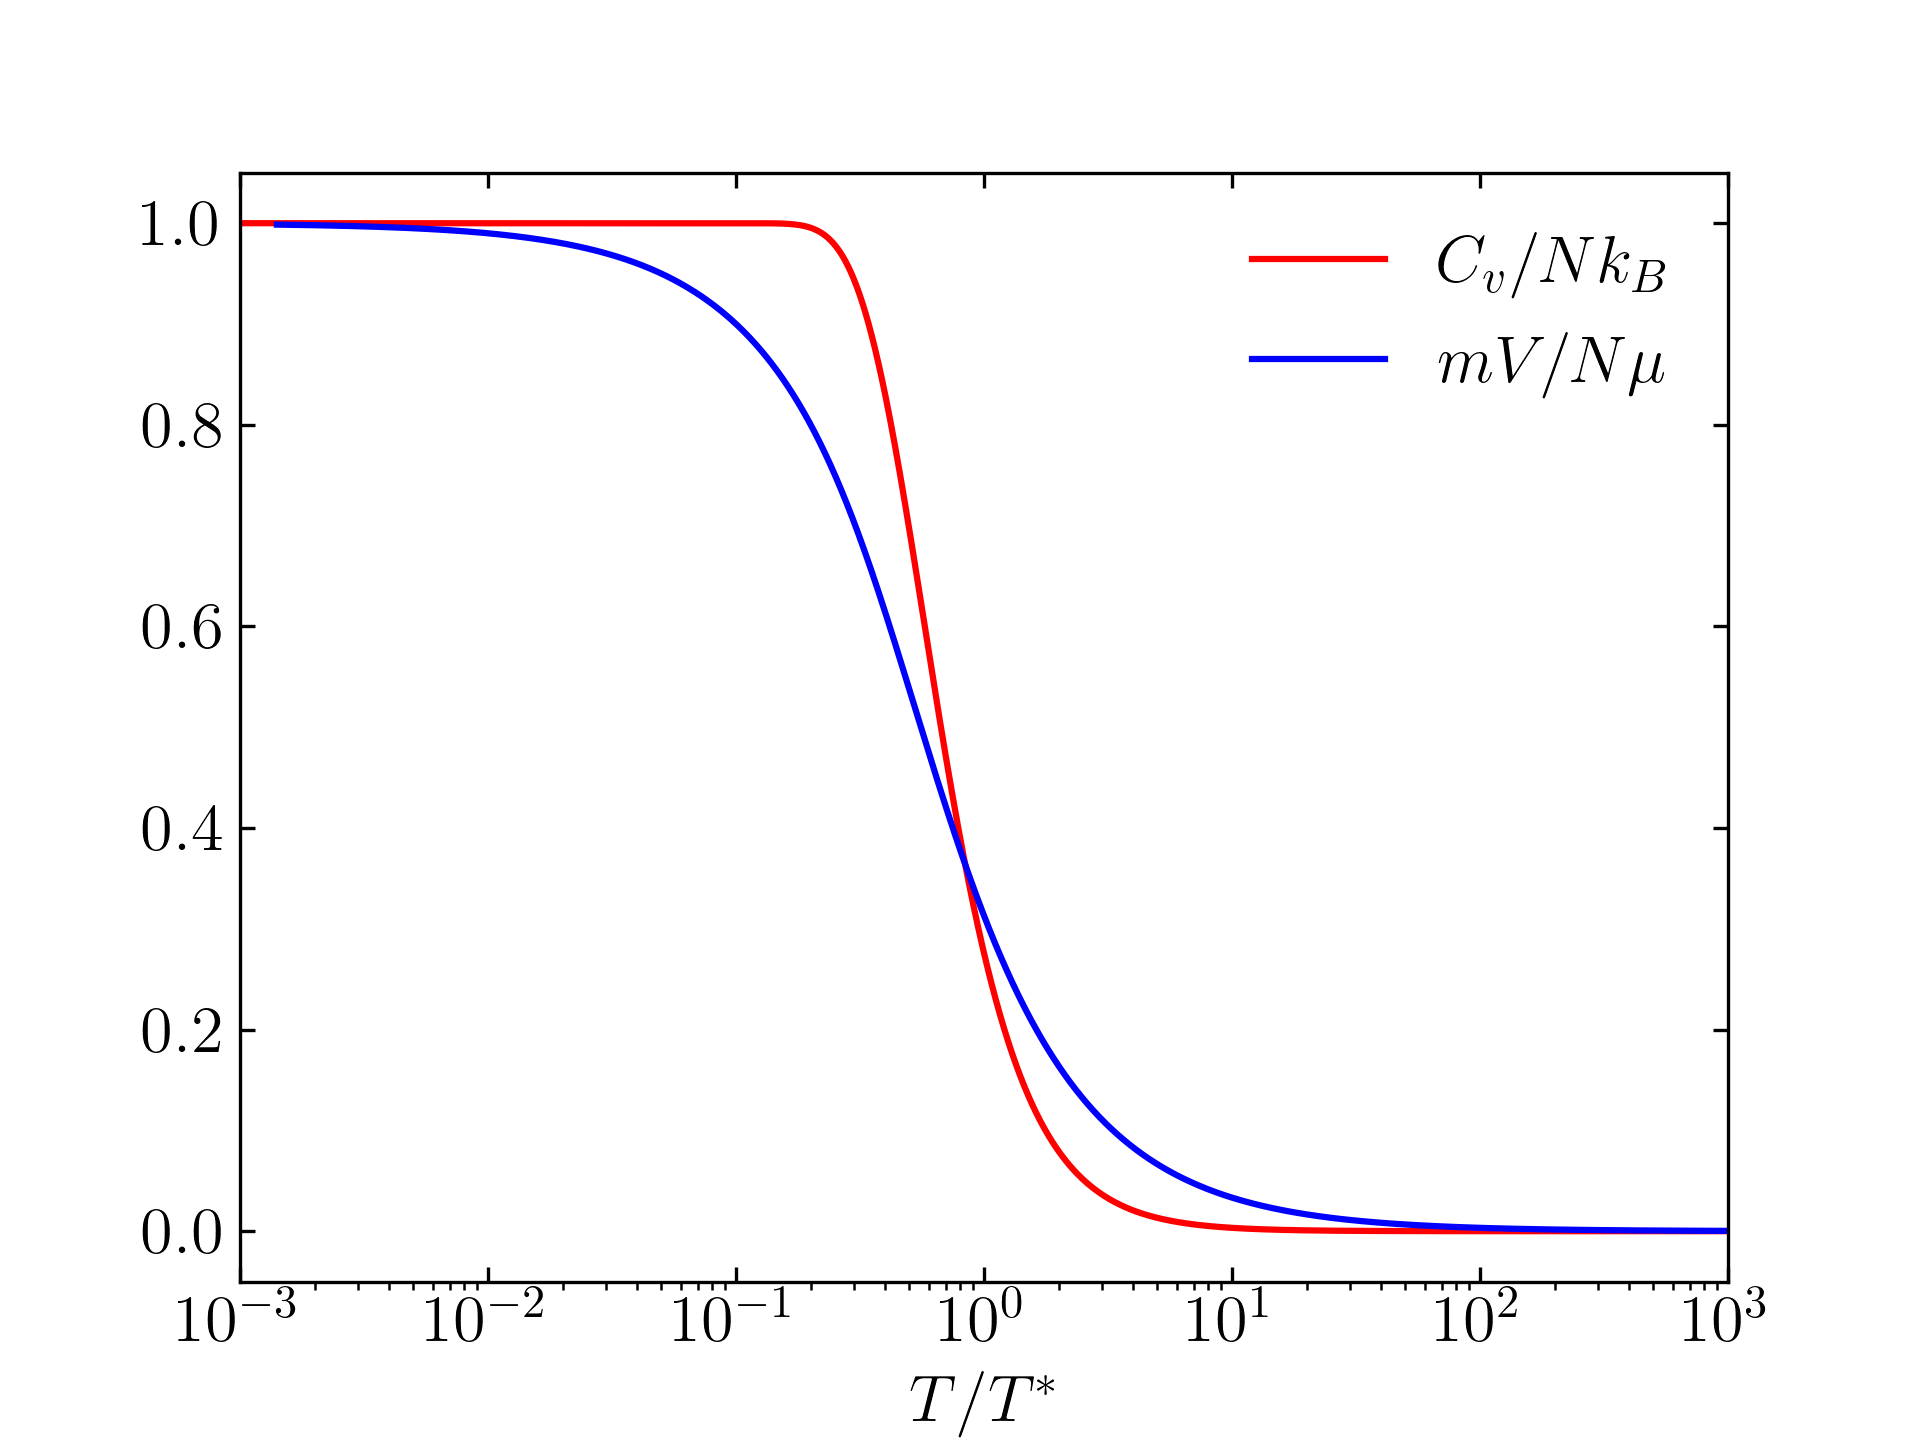
\includegraphics[width=0.8\textwidth]{p2avii.png} 
\end{center}
At low temperature, $C_v$ and $m_z$ become a constant at $Nk_B$ and $N\mu/V$,
respectively. At high temperature, both of them vanish. The cross over
temperature is $T^\ast$.

\end{solution}

(b) By noting that the magnitude of $\abs{\vb{S}}^2=S_x^2+S_y^2+S_z^2$ is fixed,
construct an argument for emergence of equipartition at \textit{low} temperature
$T$ in this classical treatment, as well as determine the corresponding
crossover temperature $T_\ast$ setting the scale below which equipartition
appears.

\begin{solution}
At low temperature, the magnetic field dominates, which generates a significant
torque on a spin. Thus, given a fixed magnitude spin $\vb{S}$ initially 
perpendicular to the field, any small perturbation from
this initial position will align the spin either parallel or anti-parallel with
the background field. Thus, each of these two states is equally probable. So, 
since there are $N$ total spins, the system has $2N$ degrees of freedom in 
which to partition the total energy. Equipartition, thus, emerges naturally at 
low temperature (or large $B$). The crossover temperature, which is
unsurprisingly determined by the field strength $B$, is already defined in
(a-vii).
\end{solution}

(c) Now repeat above calculations of (i) $F(T,B)$, (ii) $C_v(TB)$, (iii)
$m(T,B)$, (iv) $\chi(T)$ for \textit{quantum} spins $\hat{\vb{S}}_i$, each with
the magnitude fixed at $\hat{\vb{S}}^2=s(s+1)$, and microstates ranging over
$2s+1$ projection states $s_i^z=\hbar m_i$, along a quantization axis
(conveniently taken along $\vb{B}$), with $m_i\in\qty{-s,-s+1,...,s}$.
\begin{solution}

First, from Mathematica, we can calculate
\begin{align}
    Z_1
    &=\sum_{m=-s}^s\qty(e^{\mu B/k_BT})^m \notag\\
    &=\frac{e^{-sx}\qty[e^{(2s+1)x}-1]}{e^{x}-1}\tag{$x=\mu B/k_BT=\beta\mu B$}\\
    &=e^{-sx}\frac{e^{(s+1/2)x}\qty[e^{(s+1/2)x}-e^{-(s+1/2)x}]}{e^{x/2}\qty(e^{x/2}-e^{-x/2})}\notag\\
    &=\frac{\sinh\qty[(s+1/2)x]}{\sinh\qty(x/2)}.
\end{align}
Thus, we can now calculate

(i) the free energy
\begin{equation}\label{p2c:F}
    F=-Nk_BT\ln Z_1 
    =-Nk_BT\ln\qty{\frac{\sinh\qty[\beta\mu B(s+1/2)]}{\sinh\qty(\beta\mu
    B/2)}}.
\end{equation}

(ii) Let $C_1=\mu B(s+1/2)/k_B$ and $C_2=\mu B/2k_B$ so that $C_1=C_2(2s+1)$.
Then, we can differentiate $F$ in Mathematica to yield
\begin{align}
    C_v
    =-T\frac{\partial^2 F}{\partial T^2}
    =\frac{Nk_B}{T^2}
    \qty[C_2^2\csch^2\qty(\frac{C_2}{T})-C_1^2\csch^2\qty(\frac{C_1}{T})].
\end{align}
Unpacking, we can rewrite $C_v$ in meaningful variables
\begin{align}\label{p2c:Cv}
    C_v
    &=\frac{Nk_B}{T}C_2^2\qty{\csch^2\qty(\frac{1}{2}\frac{\mu
    B}{k_BT})-(2s+1)^2\csch^2\qty(\frac{2s+1}{2}\frac{\mu
    B}{k_BT})}\notag\\
    &=\frac{Nk_B}{4}\qty(\frac{\mu B}{k_BT})^2\qty{\csch^2\qty(\frac{1}{2}\frac{\mu
    B}{k_BT})-(2s+1)^2\csch^2\qty(\frac{2s+1}{2}\frac{\mu
    B}{k_BT})}\notag\\
    &=\frac{Nk_B}{4}\qty(\frac{T_1^\ast}{T})^2\qty{\csch^2\qty(\frac12\frac{T_1^\ast}{T})-(2s+1)^2\csch^2\qty(\frac{2s+1}{2}\frac{T_1^\ast}{T})},
\end{align}
where we have defined $T_1^\ast=\mu B/k_B$.

(iii) From \eqref{p2c:F}, we can calculate the energy
\begin{align}
    E
    &=F-T\frac{\partial F}{\partial T}\notag\\
    &=Nk_B\qty[C_2\coth\qty(\frac{C_2}{T})-C_1\coth\qty(\frac{C_1}{T})]\notag\\
    &=\frac{N\mu
    B}{2}\qty[\coth\qty(\frac12\frac{T_1^\ast}{T})-(2s+1)\coth\qty(\frac{2s+1}{2}\frac{T_1^\ast}{T})].
\end{align}
Then the magnetization density is
\begin{equation}\label{p2c:m}
    m=-\frac{E/B}{V}=\frac{N\mu}{2V}\qty[(2s+1)\coth\qty(\frac{2s+1}{2}\frac{T_1^\ast}{T})-\coth\qty(\frac12\frac{T_1^\ast}{T})]
    .
\end{equation}

(iv) By definition, the susceptibility is
\begin{align}\label{p2c:m}
    \chi
    &=\frac{\partial (mV)}{\partial B}\notag\\
    &=\frac{N\mu}{2}\frac{\partial}{\partial
    B}\qty[(2s+1)\coth\qty(\frac{2s+1}{2}\frac{\mu
B}{k_BT})-\coth\qty(\frac12\frac{\mu B}{k_BT})]\notag\\
    &=\frac{N\mu}{4B}\frac{T_1^\ast}{T}\qty[\csch^2\qty(\frac12\frac{T_1^\ast}{T})-(2s+1)^2\csch^2\qty(\frac{2s+1}{2}\frac{T_1^\ast}{T})].
\end{align}
\end{solution}

(d) Sketch $C_v(T,B)$ and $m(T,B)$, extract its low, intermediate, and high
temperature asymptotics, and sketch it, noting its limiting forms, two crossover
temperatures, $T_1^\ast$ and $T_2^\ast$ (discussed in the lecture) and its
connection to the classical case, that you should be able to understand by
thinking about the physics of the gaps relative to thermal energy, size of the
Hilbert space, etc. Comment on the reation to the classical treatment above.

\textit{Hint}: Note that for large $s$ (e.g., $s=10$) there are two crossover
temperatures in the quantum treatment, so three regimes that you should be able
to see for large $s$. For small $s$, e.g., $s=1/2$, the intermediate regim is
squeezed out with $T_1^\ast\approx T_2^\ast$.

\begin{solution}
From \eqref{p2c:Cv} and \eqref{p2c:m}, a plot is included below 
\begin{center}
    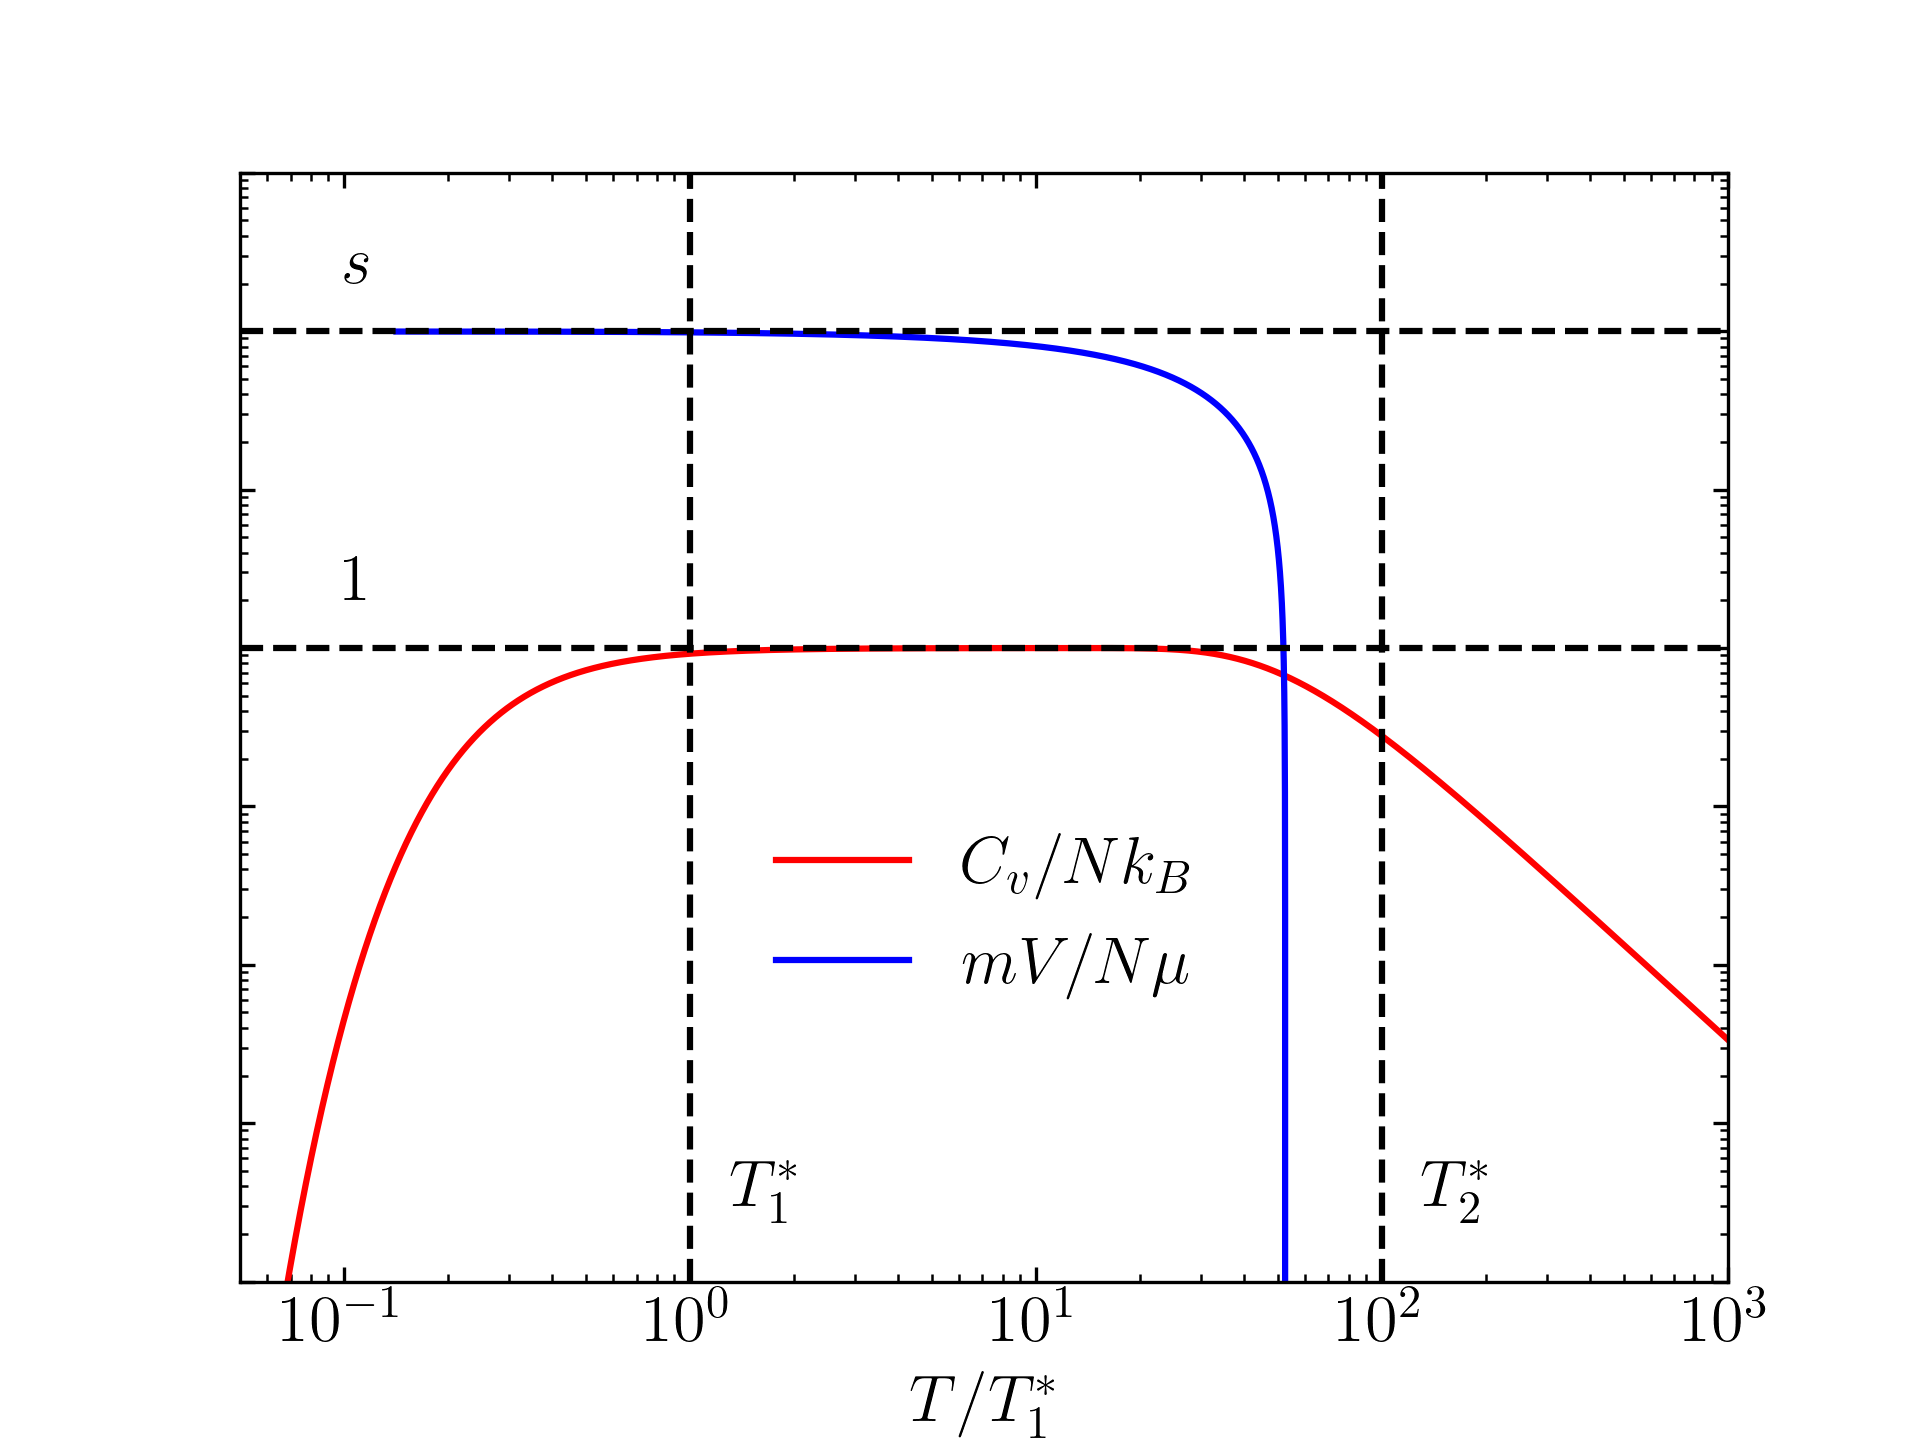
\includegraphics[width=0.8\textwidth]{p2d.png} 
\end{center}
For $T/T_1^\ast\ll1$, all spins freeze out as $C_v\to0$ and $m\to s$. Similarly,
for $T/T_2^\ast\gg 1$, $C_v\to0$ and $m\to0$, as the system approaches classical
scales. For $T_1^\ast\ll T\ll T_2^\ast$, the system does indeed have an
equipartition in energy with $C_v$ constant at $Nk_B$. The reason for this is
the same as that in the classical treatment.
\end{solution}

(e) Compute the linear magnetic susceptibility $\chi(T,B)=\eval{\partial
m/\partial B}_{B\to0}$, show that it exhibits Curie form
$\chi_\text{Curie}=c/T$, extracting the coefficient $c$.

\begin{solution}
From \eqref{p2c:m}, we take the limit
\begin{equation}
    \lim_{B\to0}\chi=\frac{N\mu^2s(s+1)}{3k_B}\frac1T.
\end{equation}
This follows Curie's law with the Curie coefficient $c=N\mu^2s(s+1)/3k_B$.
\end{solution}

(f) Show that these results reduce to those quoted in the lectures for the
simplest $s=1/2$ case. Suggestion: You will find Mathematica very useful
throughout this problem.
\begin{solution}
First, note that $\mu=g\mu_B$ with $g=2$ for spins. Now, for $s=1/2$,
\eqref{p2c:Cv} reduces to
\begin{equation}
    C_v=\frac{Nk_B}{4}\qty(\frac{T_1^\ast}{T})^2\sech^2\qty(\frac{T_1^\ast}{2T}) 
    =Nk_B\qty(\frac{T^\ast}{T})^2\sech^2\qty(\frac{T^\ast}{T}),
\end{equation}
where $T_1^\ast=\mu B/k_B=2\mu_BB/k_B=2T^\ast$. This is the same as (2.18) in my
submitted HW1. Similarly, \eqref{p2c:m} reduces to
\begin{equation}
    m=\frac{N\mu}{2V}\qty[2\coth\qty(\frac{2T^\ast}{T})-\coth\qty(\frac{T^\ast}{T})]
    =\frac{N\mu_B}{V}\tanh\qty(\frac{T^\ast}{T}),
\end{equation}
which is (2.12) in my HW1. Finally, the linear susceptibility reduces to
\begin{equation}
    \chi_\text{linear}=\frac{N4\mu_B^2\frac{3}{4}}{3k_B}\frac1T
    =\frac{N\mu_B^2}{k_B}\frac1T,
\end{equation}
which is the same as (2.15) in my HW1.
\end{solution}
\end{problem}
\newpage
%%%%%%%%%%%%%%%%%%%%%%%%%%%%%%%%%%%%%%%%%%%%%%%%%%%%%%%%%%%%%%%%%%%%%%%%%%%%%%%
%%%%%%%%%%%%%%%%%%%%%%%%%%%%%%%%%%%%%%%%%%%%%%%%%%%%%%%%%%%%%%%%%%%%%%%%%%%%%%%
\begin{problem}{3}[Gaussian integrals calculus]
In most problems throughout statistical mechanics, key component of computations
involves Gaussian integration over degrees of freedom, with this, amazingly even
extending to quantum statistical mechanics, thanks to the Feynman's path
integral formulation. Thus, one needs to become fluent with Gaussian integrals
calculus as we will do with the problems below.

(a) Derive standard moments of a Gaussian distribution
\begin{subequations}
    \begin{align}
        Z_0(a)&=\int_{-\infty}^\infty dx
        e^{-ax^2/2}=\sqrt{\frac{2\pi}{a}},\label{p3a:Z0}\\
        Z_1(a)&=\int_{-\infty}^\infty dxx^2
        e^{-ax^2/2}=\frac1a\sqrt{\frac{2\pi}{a}}=\frac1aZ_0,\label{p3a:Z1}\\
        Z_n(a)&=\int_{-\infty}^\infty dx
        x^{2n}e^{-ax^2/2}=\frac{(2n-1)!!}{a^n}Z_0,\label{p3a:Zn}
    \end{align}
\end{subequations}
that can be deduced from dimensional analysis, relation to the first basic
``partition function'' integral $Z_0(a)$ (that can in turn be computed by a
standard trick of squaring it and integrating in polar coordinates) or another
generating function (see below) and $\Gamma$-functions.

\begin{solution}
First, squaring \eqref{p3a:Z0} yields
\begin{align}
    Z_0^2
    &=\qty(\int_{-\infty}^\infty dxe^{-ax^2/2})\qty(\int_{-\infty}^\infty
    dye^{-ay^2/2})\notag\\
    &=\int_{-\infty}^\infty\int_{-\infty}^\infty dxdy
    e^{-ar^2/2}\tag{$r^2=x^2+y^2$}\\
    &=\int_0^\infty\int_0^{2\pi}rdrd\theta
    e^{-ar^2/2}\tag{$x=r\cos\theta,y=r\sin\theta$}\\
    &=\frac{2\pi}{a}\int_0^\infty du e^{-u}\tag{$u=ar^2/2$}\\
    &=\frac{2\pi}{a}.
\end{align}
Thus, it follows that $Z_0=\sqrt{2\pi/a}$, as in \eqref{p3a:Z0}. Now,
differentiating both sides of \eqref{p3a:Z0} yields
\begin{equation}
    -\frac1{2a}\sqrt{\frac{2\pi}{a}}=\int_{-\infty}^\infty
    dx\qty(-\frac{x^2}{2})e^{-ax^2/2}=-\frac12Z_1
    \Rightarrow Z_1=\frac1a\sqrt{\frac{2\pi}{a}}=\frac1aZ_0.
\end{equation}
Having proven the base case \eqref{p3a:Z1}, we can prove that \eqref{p3a:Zn} is
true for any $n\in\N$ by induction. Suppose the induction hypothesis (the
case $n-1\in\N$), is true, or in other words, that
\begin{equation}
    Z_{n-1}=\int_{-\infty}^\infty dx x^{2n-2}e^{-ax^2/2}
    =\frac{(2n-3)!!}{a^{n-1}}Z_0.
\end{equation}
On one hand, differentiating the RHS of the second equality gives
\begin{equation}\label{p3a:RHS}
    \frac{\partial Z_{n-1}}{\partial
    a}=-\frac1{2a^n}\sqrt{\frac{2\pi}{a}}(2n-1)(2n-3)!!
    =-\frac{(2n-1)!!}{2a^n}Z_0.
\end{equation}
On the other hand, differentiating the LHS of the second equality gives
\begin{equation}\label{p3a:LHS}
    \frac{\partial Z_{n-1}}{\partial a}
    =\int_{-\infty}^\infty dxx^{2n-2}\qty(-\frac12x^2)e^{-ax^2/2}
    =-\frac12\int_{-\infty}^\infty dxx^{2n}e^{-ax^2/2}
    =-\frac12Z_{n}.
\end{equation}
Combining \eqref{p3a:RHS} and \eqref{p3a:LHS} yields
\begin{equation}
    Z_n=\frac{(2n-1)!!}{a^n}Z_0 .
\end{equation}
Thus, we are done proving \eqref{p3a:Zn}.
\end{solution}

(b) Show that these moments can also be obtained from the generating function
$Z(a,h)$ by differentiating with respect to ``external field'' $h$:
\begin{align}
    Z(a,h)&=\int_{-\infty}^\infty dx
    e^{-ax^2/2+hx}=Z_0(a)e^{h^2/2a},\label{p3b:Za}\\
          &=\sum_{n=0}^\infty\frac{h^{2n}}{(2n)!}Z_n(a).
\end{align}

\begin{solution}
First, define the generating function
\begin{align}
    Z(a,h)
    &=\int_{-\infty}^\infty dx e^{-ax^2/2+hx} \notag\\
    &=e^{h^2/2a}\int_{-\infty}^\infty dxe^{-ax^2/2+hx-h^2/2a}\notag\\
    &=e^{h^2/2a}\int_{-\infty}^\infty dxe^{-a(x^2-2hx/a+h^2/a^2)/2}\notag\\
    &=e^{h^2/2a}\int_{-\infty}^\infty dxe^{-a(x-h/a)^2/2}\notag\\
    &=e^{h^2/2a}\int_{-\infty}^\infty due^{-au^2/2}\tag{$u=x-h/a$}\notag\\
    &=e^{h^2/2a}Z_0(a)\notag\\
    &=Z_0(a)\sum_{k=0}^{\infty}\frac1{k!}\frac{h^{2k}}{(2a)^k}.
\end{align}
where we have used the series expansion of $e^{x}$ in the last equality. By
definition, we can relate $Z_n$ to the generating function $Z$ by
\begin{align}\label{p3b:Zn}
    Z_n=\eval{\frac{\partial^{2n} Z}{\partial h^{2n}}}_{h=0}
    =Z_0(a)\sum_{k=0}^\infty
    \frac1{k!}\frac1{2^ka^k}\eval{\frac{\partial^{2n}}{\partial
    h^{2n}}\qty(h^{2k})}_{h=0}.
\end{align}
Now, the terms $k<n$ in the series trivially vanish, since the polynomial
$h^{2k}$ is differentiated more than $2k$ times. Then \eqref{p3b:Zn} becomes
\begin{align}
    Z_n
    =Z_0(a)\frac{(2n)!}{2^nn!}\frac1{a^n}
    +Z_0(a)\sum_{k=n+1}^\infty\frac{1}{k!2^ka^k}\eval{\frac{\partial^{2n}}{\partial
    h^{2n}}\qty(h^{2k})}_{h=0}
    =Z_0(a)\frac{(2n-1)!!}{a^n}.
\end{align}
The series in the first equality vanishes because the polynomials
$\partial^{2n}(h^{2k})/\partial h^{2n}$ with non-trivial powers of $h$ are
evaluated at $h=0$. We then obtain the same result in \eqref{p3a:Zn}.
\end{solution}


(c) Now use Gaussian integral calculus to derive statistical mechanics for a
classical 1D harmonic oscillator under an external force, $f$, with a
Hamiltonian $\HH=p^2/2m+(1/2)m\omega^2x^2-fx$, by computing

\qquad(i) its free energy, $F(T)$,

\qquad(ii) expectation values $\expval{x},\expval{x^2},\expval{p^2}$,

\qquad(iii) standard deviation
$\sqrt{\expval{(x-\expval{x})^2}}=\sqrt{\expval{x^2}-\expval{x}^2}$, also
demonstrating the last equality.

\begin{solution}
By definition, the partition function is
\begin{align}
    Z
    &=\frac1{2\pi\hbar}\int_{-\infty}^\infty\int_{-\infty}^\infty dx dp
    \exp\qty(-\frac12\frac{\beta}{m}p^2-\frac12\beta m\omega^2x^2+\beta
    fx)\notag\\
    &=\frac1{2\pi\hbar}\sqrt{\frac{2\pi}{\beta/m}}\sqrt{\frac{2\pi}{\beta
    m\omega^2}}e^{\beta f^2/2m\omega^2}\notag\\
    &=\frac1{\hbar\omega\beta}e^{\beta f^2/2m\omega^2}.
\end{align}

(i) Then, the free energy is
\begin{equation}
    F=-k_BT\ln Z=-\frac{f^2}{2m\omega^2}-k_BT\ln\qty(\frac{k_BT}{\hbar\omega}) 
\end{equation}

(ii) First, note from \eqref{p3b:Za} that
\begin{equation}
    \int_{-\infty}^\infty dx xe^{-ax^2/2+hx}
    =Z_0\frac{h}{a}e^{h^2/2a},
    \qquad
    \text{and}
    \qquad
     \int_{-\infty}^\infty dx x^2e^{-ax^2/2+hx}
    =Z_0\qty(\frac1a+\frac{h^2}{a^2})e^{h^2/2a}.
\end{equation}
We can then use these results to calculate
\begin{align}
    \expval{x}
    &=\frac1Z\frac1{2\pi\hbar}\int_{-\infty}^\infty
    dp\exp\qty(-\frac12\frac\beta{m}p^2)
    \int_{-\infty}^\infty dx x\exp\qty(-\frac12\beta m\omega^2x^2+\beta
    fx)\notag\\
    &=\frac1Z\frac{1}{2\pi\hbar}\sqrt{\frac{2\pi}{\beta/m}}
    \sqrt{\frac{2\pi}{\beta m\omega^2}}\frac{f}{m\omega^2}e^{\beta
    f^2/2m\omega^2}\notag\\
    &=\frac{f}{m\omega^2}.
\end{align}
Similarly, 
\begin{align}
    \expval{x^2}
    &=\frac1Z\frac1{2\pi\hbar}
    \int_{-\infty}^\infty dp\exp\qty(-\frac12\frac\beta{m}p^2)
    \int_{-\infty}^\infty dx x^2\exp\qty(-\frac12\beta m\omega^2x^2+\beta
    fx)\notag\\
    &=
    \frac1Z\frac1{2\pi\hbar}\sqrt{\frac{2\pi}{\beta/m}}
    \sqrt{\frac{2\pi}{\beta m\omega ^2}}\qty(\frac1{\beta
    m\omega^2}+\frac{f^2}{m^2\omega^4})e^{\beta
f^2/2m\omega^2}\notag\\
    &=\frac1{\beta m\omega^2}+\frac{f^2}{m^2\omega^4},
\end{align}
and
\begin{align}
     \expval{p^2}
    &=\frac1Z\frac1{2\pi\hbar}
    \int_{-\infty}^\infty dpp^2\exp\qty(-\frac12\frac\beta{m}p^2)
    \int_{-\infty}^\infty dx \exp\qty(-\frac12\beta m\omega^2x^2+\beta
    fx)\notag\\
    &=\frac1Z\frac1{2\pi\hbar}\frac{m}{\beta}\sqrt{\frac{2\pi}{\beta/m}}
    \sqrt{\frac{2\pi}{\beta m\omega^2}}e^{\beta f^2/2m\omega^2}\notag\\
    &=\frac{m}{\beta}.
\end{align}

(iii) By definition, the standard deviation is
\begin{align}
    \sigma_x
    &=\sqrt{\expval{(x-\expval{x})^2}}\notag\\
    &=\sqrt{\expval{(x-f/m\omega^2)^2}}\notag\\
    &=\sqrt{\expval{x^2}-2(f/m\omega^2)\expval{x}+f^2/m^2\omega^4}\notag\\
    &=\frac1{\sqrt{\beta m\omega^2}}.
\end{align}
Also, we can calculate it with
\begin{align}
    \sigma_x
    &=\sqrt{\expval{x^2}-\expval{x}^2}\notag\\
    &=\sqrt{\frac1{\beta
    m\omega^2}+\frac{f^2}{m^2\omega^4}-\frac{f^2}{m^2\omega^4}}\notag\\
    &=\frac1{\sqrt{\beta m\omega^2}},
\end{align}
which gives the same result.
\end{solution}

(d) Generalize above results to $N$ quadratic variables, corresponding to
coupled Gaussian integrals characterized by an $N\times N$ symmetric matrix
$(\vb{A})_{ij}$, as would appear in a Hamiltonian for $N$ coupled harmonic
oscillators,
\begin{subequations}
    \begin{align}
        Z_0(\vb{A})&=\int_{-\infty}^\infty
        \qty[d\vb{x}]e^{-(1/2)\vb{x}^T\vdot\vb{A}\vb{x}}=\prod_{i=1}^N\sqrt{\frac{2\pi}{a_i}}=\sqrt{\frac{(2\pi)^N}{\det\vb{A}}},
        \\
        Z_1^{ij}(\vb{A})
                   &=\int_{-\infty}^\infty
                   \qty[d\vb{x}]x_ix_je^{-(1/2)\vb{x}^T\vdot\vb{A}\vdot\vb{x}}=\vb{A}_{ij}^{-1}Z_0,\\
                   Z(\vb{A},\vb{h})
                   &=\int_{-\infty}^\infty\qty[d\vb{x}]
                   e^{-(1/2)\vb{x}^T\vdot\vb{A}\vdot\vb{x}+\vb{h}^T\vdot\vb{x}}
                   =e^{(1/2)\vb{h}^T\vdot\vb{A}^{-1}\vdot\vb{h}}Z_0,
    \end{align} 
\end{subequations}
computed by diagonalizing the symmetric matrix $\vb{A}$ and thereby decoupling
the $N$-dimensional integral into a product of $N$ independent scalar Gaussian
integrals \eqref{p3a:Zn}, each characterized by eigenvalue $a_i$, and then
converting back into representation-independent form. In above, we also define a
common multi-integral notation
$\int_{-\infty}^\infty\qty[d\vb{x}]=\prod_{i=1}^N\qty[\int_{-\infty}^\infty
dx_i]$.

\begin{solution}
First, since $\vb{A}$ is symmetric, the spectral theorem states that there
exists an orthogonal transformation $\vb{C}$ such that
$\tilde{\vb{A}}=\vb{C}\vdot\vb{A}\vdot\vb{C}^T=\text{diag}(a_1,...,a_N)$ is a diagonal
matrix where $a_i$ are the eigenvalues. Let $\vb{y}=\vb{C}\vdot\vb{x}$ be a
vector in the new basis. Then it follows that
\begin{equation}
    \vb{x}^T\vdot\vb{A}\vdot\vb{x}
    =\vb{x}^T\vdot\vb{C}^T\vdot\tilde{\vb{A}}\vdot\vb{C}\vdot\vb{x}
    =\vb{y}^T\vdot\tilde{\vb{A}}\vdot\vb{y}
    =\sum_{i=1}^Na_iy_i^2.
\end{equation}
Also, since $\vb{C}$ is orthogonal, $d\vb{x}=\norm{J\vb{C}}d\vb{y}=d\vb{y}$
where $J\vb{C}$ is its Jacobian. Finally, we can compute
\begin{align}
    Z_0
    =\int_{-\infty}^\infty\qty[d\vb{y}]
    \exp\qty(-\sum_{i=1}^Na_iy_i^2/2)
    =\prod_{i=1}^N\qty[\int_{-\infty}^\infty e^{-a_iy_i^2/2}]
    =\prod_{i=1}^N\sqrt{\frac{2\pi}{a_i}}
    =\sqrt{\frac{(2\pi)^N}{\det\vb{A}}}.
\end{align}
where $\det\vb{A}=\prod_{i=1}^Na_i$.


Now, from matrix multiplication, the components of $\vb{x}=\vb{C}^T\vdot\vb{y}$
are
\begin{equation}
    x_i=\sum_{k=1}^NC_k^Ty_k .
\end{equation}
It then follows that
\begin{align}
    Z_1^{ij}
    &=\int_{-\infty}^\infty\qty[d\vb{y}]
    \qty(\sum_{k=1}^NC_{ik}^Ty_k)\qty(\sum_{l=1}^NC_{jl}^Ty_l)
    \exp\qty(-\sum_{n=1}^N\frac12a_ny_n^2)\notag\\
    &=\sum_{k,l=1}^NC_{ik}^TC_{lj}\prod_{n=1}^\infty
        \int_{-\infty}^\infty dy_n y_ky_le^{-a_ny_n^2/2}\notag\\
    &=\sum_{k=1}^NC_{ik}^TC_{kj}\prod_{i=1}^N\int_{-\infty}^\infty
    dy_ny_k^2e^{-a_ny_n^2/2}\notag\\
    &=\sum_{k=1}^\infty C_{ik}^TC_{jk}\frac1{a_k}\sqrt{\frac{2\pi}{a_k}}
    \sqrt{\frac{(2\pi)^{N-1}}{\det\vb{A}/a_k}}\notag\\
    &=Z_0\sum_{k=1}^\infty C_{ik}^T\frac1{a_k}C_{kj}\notag\\
    &=Z_0\qty(\vb{C}^T\vdot\tilde{\vb{A}}^{-1}\vdot\vb{C})_{ij}\notag\\
    &=Z_0\qty(\vb{C}^T\vdot\tilde{\vb{A}}\vdot\vb{C})_{ij}^{-1}\notag\\
    &=Z_0\vb{A}_{ij}^{-1}
\end{align}
where we have used the fact that $\vb{C}^T=\vb{C}^{-1}$ because $\vb{C}$ is
orthogonal.

Finally, note that
\begin{equation}
    \vb{h}^T\vdot\vb{A}^{-1}\vdot\vb{h}
    =\vb{h}^T\vdot\vb{C}^T\vdot\tilde{\vb{A}}^{-1}\vdot\vb{C}\vdot\vb{h}
    =\tilde{\vb{h}}^T\vdot\tilde{\vb{A}}^{-1}\tilde{\vb{h}}
    =\sum_{i=1}^N\frac{\tilde{h}_i^2}{a_i}
\end{equation}
where $\tilde{\vb{h}}=\vb{C}\vdot\vb{h}$.  Then, we can compute
\begin{align}
    -\frac12\vb{x}^T\vdot\vb{A}\vdot\vb{x}+\vb{h}^T\vdot\vb{x}
    &=-\frac12\vb{y}^T\tilde{\vb{A}}\vdot\vb{y}
    +\vb{h}^T\vdot\vb{C}^T\vdot\vb{y}
    -\frac12\tilde{\vb{h}}\vdot\tilde{\vb{A}}^{-1}\vdot\tilde{\vb{h}}
    +\frac12\tilde{\vb{h}}\vdot\tilde{\vb{A}}^{-1}\vdot\tilde{\vb{h}}
    \notag\\
    &=\sum_{i=1}^N\qty[\frac{\tilde{h}_i^2}{a_i}-\frac12a_i\qty(y_i-\frac{\tilde{h}_i}{a_i})^2],
\end{align}
and so
\begin{align}
    Z(\vb{A},\vb{h})
    &=\exp\qty(\sum_{i=1}^{N}\tilde{h}_i^2/a_i)
    \prod_{i=1}^N\int_{-\infty}^\infty
    dy_i\exp\qty[-\frac12a_i\qty(y_i-\frac{\tilde{h}_i}{a_i})^2]\notag\\
    &=e^{-(1/2)\vb{h}^T\vdot\vb{A}^{-1}\vdot\vb{h}}
    \prod_{i=1}^N\int_{-\infty}^\infty
    d\overline{y}_i\exp\qty(-\frac12a_i\overline{y}_i^2)\tag{$\overline{y}_i=y_i-\tilde{h}_i/a_i$}\\
    &=e^{-(1/2)\vb{h}^T\vdot\vb{A}^{-1}\vdot\vb{h}}Z_0
\end{align}
\end{solution}

(e) As a corollary of these Gaussian integral identities, demonstrate two more
key results for a Gaussian random variable $\vb{x}$ (obeying Gaussian
statistics), with variance $\vb{A}_{ij}^{-1}$,
\begin{align}
    Z\qty[\vb{h}]&\equiv\expval{e^{\vb{h}^T\vdot\vb{x}}}Z_0
    =e^{(1/2)\expval{\qty(\vb{h}^T\vdot\vb{x})^2}}Z_0
    =e^{(1/2)\vb{h}^T\vdot\vb{G}\vdot\vb{h}}Z_0,\\
    \expval{\vb{x}_i\vb{x}_j}
                 &\equiv
                 G_{ij}^0=\frac1{Z_0}\int_{-\infty}^\infty\qty[d\vb{x}]x_ix_je^{-(1/2)\vb{x}^T\vdot\vb{A}\vdot\vb{x}}
                 =\vb{A}_{ij}^{-1},\\
                 &=\frac1{Z_0}\frac{\partial^2}{\partial h_i\partial
             h_j}\eval{Z\qty[\vb{h}]}_{\vb{h}=0}
             =\frac{\partial^2}{\partial h_i\partial h_j}\ln
             \eval{Z[\vb{h}]}_{\vb{h}=0}
\end{align}
with the first identity the relative of the so-called Wick's theorem in field
theory, which is extremely important for computation of Gaussian correlation
functions. $Z\qty[\vb{h}]$ is called the generating function for corelators of
$\vb{x}$, because its $n$-th derivative wrt $h_i$ gives $n$-point correlation
function of $x_i$. 

Note: As we saw in lecture and will study below, application these identities to
systems with quadratic degrees of freedom immediately reproduces the
equipartition theorem ($\frac12k_BT$ per classical quadratic degree of freedom),
as in e.g., phonons in a solid or free particles of the Boltzmann gas.

\end{problem}
\newpage
%%%%%%%%%%%%%%%%%%%%%%%%%%%%%%%%%%%%%%%%%%%%%%%%%%%%%%%%%%%%%%%%%%%%%%%%%%%%%%%
%%%%%%%%%%%%%%%%%%%%%%%%%%%%%%%%%%%%%%%%%%%%%%%%%%%%%%%%%%%%%%%%%%%%%%%%%%%%%%%
\begin{problem}{4}[Quantum harmonic oscillators: Einstein solid]
Let's revisit the problem of $N$ decoupled 3D quantum harmonic oscillators as a
model of atomic vibrations in a crystalline solid (Einstein phonons), described
by familiar quantum Hamiltonian
\begin{equation}
    \HH=\sum_{i}^N
    \qty[\frac{\hat{\vb{p}}_i^2}{2m}
    +\frac12m\omega_0^2\hat{\vb{r}}_i^2-\frac32\hbar\omega_0] 
\end{equation}
where for convenience I defined $\HH$ with zero point energy subtracted off. We
now will treat this probem within canonical ensemble formalism to be compared
and contrasted with its earlier treatment with microcanonical ensemble.

(a) Recalling the eigenvalues
$E[\qty{n_\alpha}]=\hbar\omega_0\sum_{\alpha=1}^{3N}n_\alpha$
($\alpha=x_1,y_1,z_1,\hdots,$ ranging from 1 to $3N$) for the harmonic
oscillator Hamiltonian, compute the partition function
\begin{equation}
    Z(T)=\sum_{\qty{n_\alpha}}e^{-\beta E\qty[\qty{n_\alpha}]}.
\end{equation}
\textit{Hint}: Here and throughout, note that $Z_n=Z_1^N$, with many simiarly
simplifying properties that follow, since oscillators are decoupled. That's what
makes decoupled modes so simple, reducng an $N$-mode problem to that of a single
mode.
\begin{solution}
By definition, the partition function is
\begin{align}
    Z
    &=\sum_\qty{n}\exp\qty(-\beta\hbar\omega_0\sum_{\alpha=1}^{3N}n_\alpha) \notag\\
    &=\prod_{\alpha=1}^{3N}\qty[\sum_\qty{n_\alpha}\exp\qty(-\beta\hbar\omega_0n_\alpha)]\notag\\
    &=\qty[\sum_{n_\alpha=0}^\infty\exp\qty(-\beta\hbar\omega_0n_\alpha)]^{3N}\notag\\
    &=\qty(\frac{e^{x}}{e^x-1})^{3N}\tag{$x=\hbar\omega_0/k_BT$}\\
    &=\qty(\frac{e^{x/2}}{e^{x/2}-e^{-x/2}})^{3N}\notag\\
    &=\qty[\frac{e^{\hbar\omega_0/2k_BT}}{2\sinh\qty(\hbar\omega_0/2k_BT)}]^{3N},
\end{align}
where we have used Mathematica to calculate the geometric series in the third
equality.
\end{solution}

(b) Compute the entropy $S(T)$ and the corresponding average energy $E(T)$,
exploring its classical $\hbar\omega_0/k_BT\ll 1$ and quantum
$\hbar\omega_0/k_BT\gg 1$ limiting functional forms.

\begin{solution}
It follows from part (a) that the free energy is
\begin{equation}
    F=-3Nk_BT\ln\qty[\frac{e^{\hbar\omega_0/2k_BT}}{2\sinh\qty(\hbar\omega_0/2k_BT)}]
    =3N\qty{k_BT\ln\qty[2\sinh\qty(\frac{\hbar\omega_0}{2k_BT})]-\frac{\hbar\omega_0}{2}}.
\end{equation}
The entropy is then (plugging into Mathematica),
\begin{equation}
    S=-\frac{\partial F}{\partial T}
    =3Nk_B\qty{\frac{\hbar\omega_0}{2k_BT}\coth\qty(\frac{\hbar\omega_0}{2k_BT})-\ln\qty[2\sinh\qty(\frac{\hbar\omega_0}{2k_BT})]}.
\end{equation}
And the energy is
\begin{equation}
    E=F+TS
    =\frac32N\hbar\omega_0\qty[\coth\qty(\frac{\hbar\omega_0}{2k_BT})-1].
\end{equation}
At low temperature ($T\to0$), $x\to\infty$ and $\coth(x)\to1$. Thus, $E\to0$. At
high temperature, $x\to0$ and we can Taylor expand $\coth(x)\approx
1/x+x/3\to1/x$ and the energy is
\begin{equation}\label{p4b:E}
    E(x\to0)=\frac32N\hbar\omega_0\qty(\frac{2k_BT}{\hbar\omega_0}-1)
    =3Nk_BT\qty(1-x)\approx3Nk_BT.
\end{equation}
Both of these limits are the same as those found in HW1.
\end{solution}

(c) Compute the heat capacity $C_v(T)=T\partial S/\partial T=\partial E/\partial
T$ and explore its classical (high $T$) and quantum (low $T$) limits, showing
the expected equipartition $C_v=N_\text{dof}k_B$ in the former and its breakdown
in the latter limits. Plot $C_v(T)$, noting the crossover temperature and
limiting forms.
\begin{solution}
From \eqref{p4b:E}, we can calculate
\begin{equation}
    C_v=\frac{\partial E}{\partial T}
    =\frac{3N}{4}\qty(\frac{\hbar\omega_0}{k_BT})^2\csch^2\qty(\frac{\hbar\omega_0}{2k_BT})
=3N\qty(\frac12\frac{T^\ast}{T})^2\csch^2\qty(\frac12\frac{T^\ast}{T})
\end{equation}
where we have defined the crossover temperature $T^\ast=\hbar\omega_0/k_B$. A
plot is included below
\begin{center}
    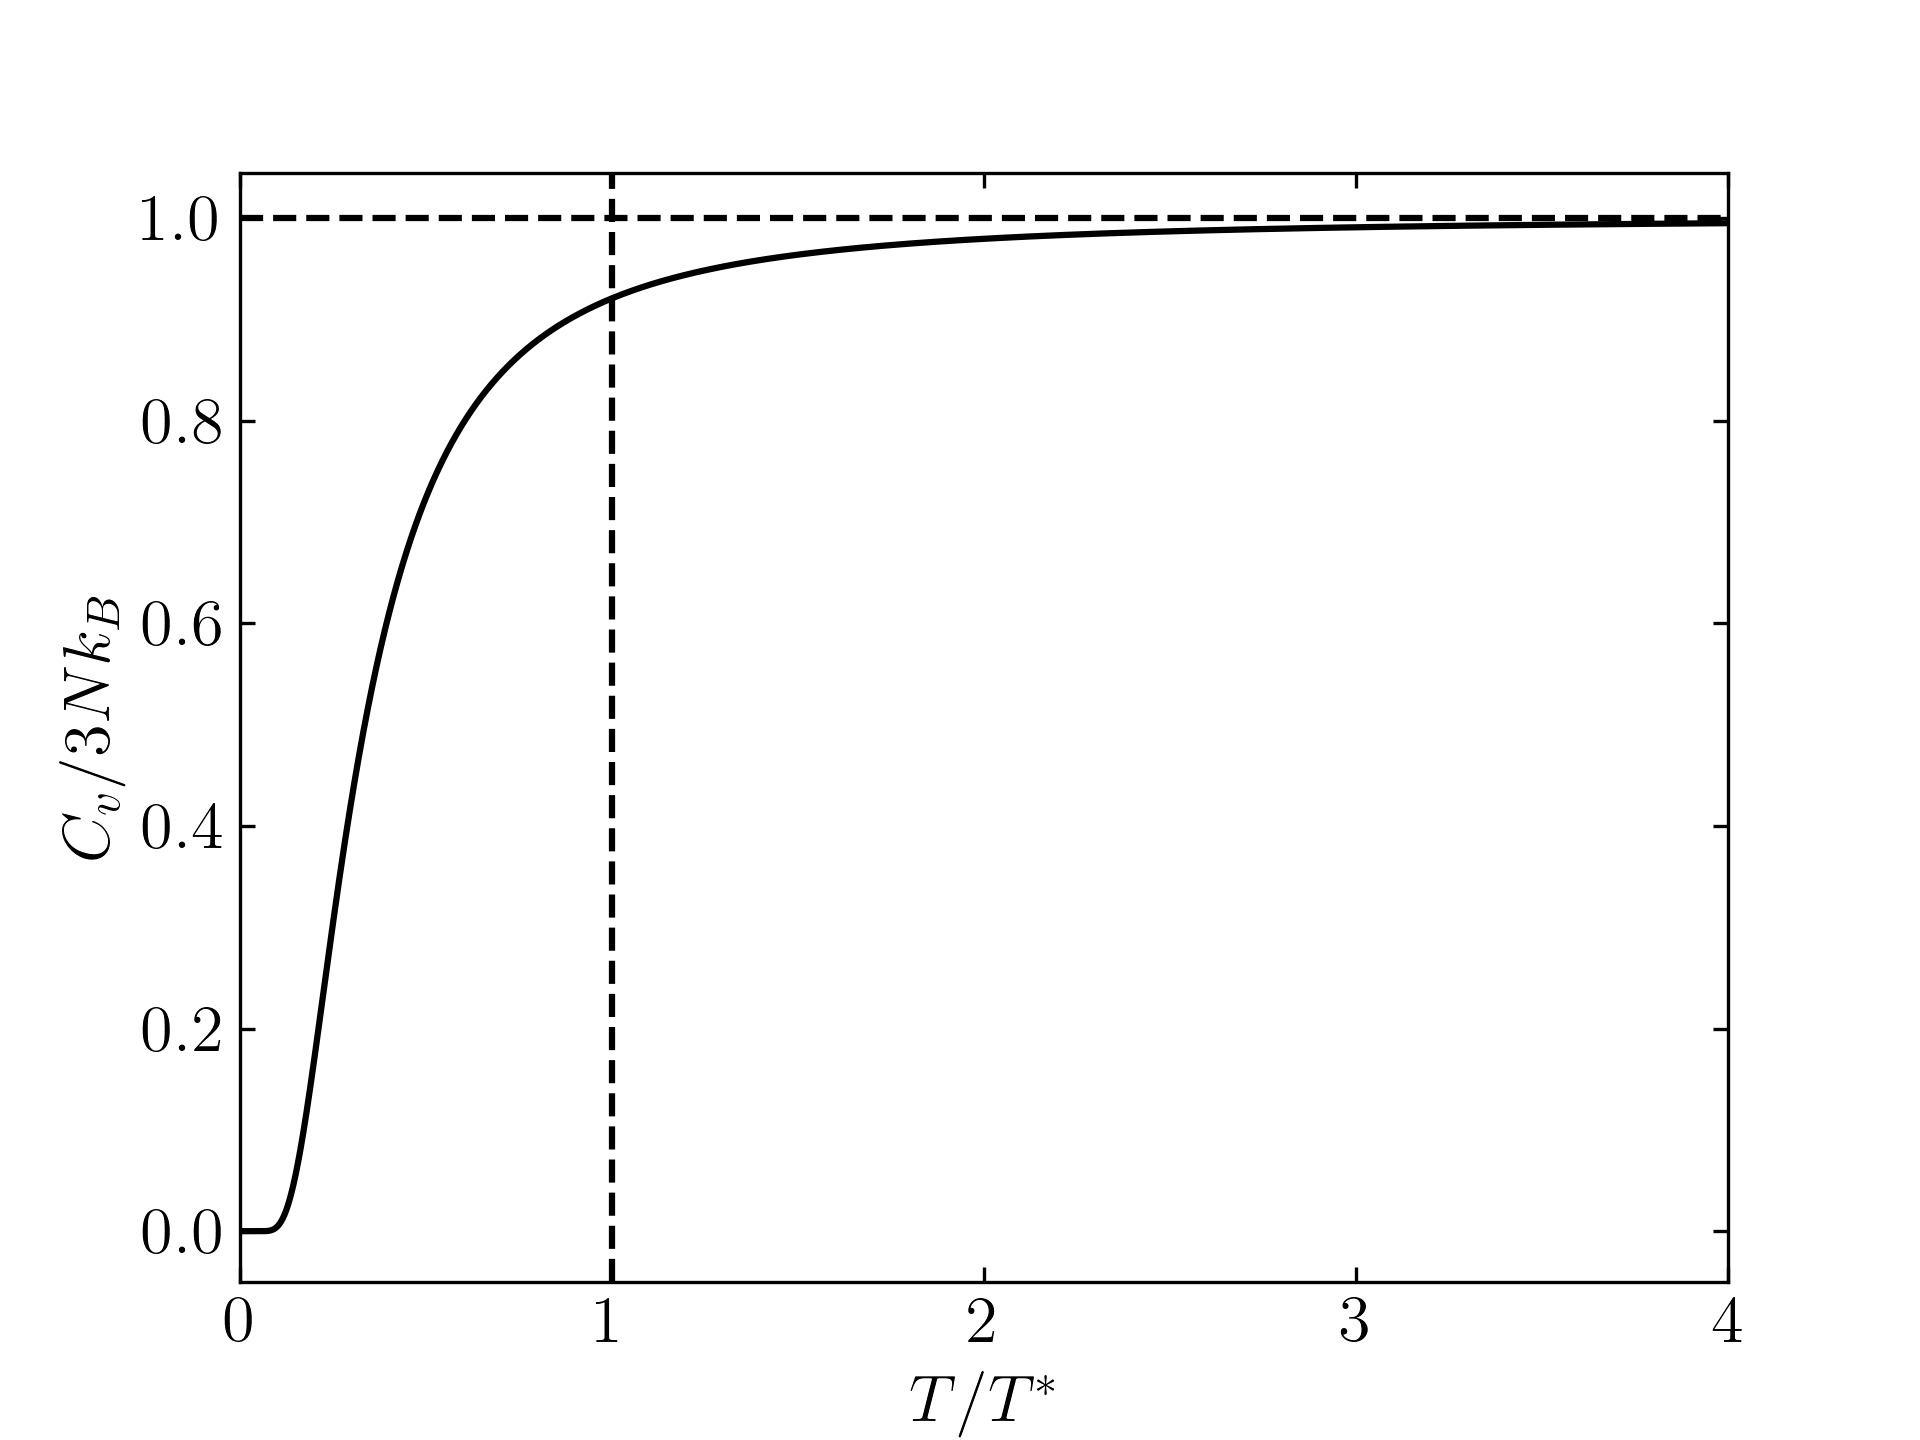
\includegraphics[width=0.8\textwidth]{p4c.png} 
\end{center}
In the classical limit ($T\to\infty$), $x\to0$ and $x^2\csch^2(x)\to1$.
Thus, equipartition emerges with $C_v=3Nk_B$ where $3N=N_\text{dof}$. In the
quantum limit ($T\to0$), $x\to\infty$ and $x^2\csch^2(x)\to0$. The system
freezes out. This is the same results as in HW1.
\end{solution}

(d) Consider a classical limit of the problem with small $\hbar\omega_0/k_BT$
such that $E\qty[\qty{n_\alpha}]=\sum_{\alpha=1}^{3N}\epsilon_\alpha$ and
oscillator eigenvalues $\epsilon_\alpha$ vary nearly continuously. Using this
simplification compute
\begin{equation}
    Z(T)=\prod_{\alpha=1}^{3N}\int\frac{d\epsilon_\alpha}{\hbar\omega_0}e^{-\beta
    E[\qty{\epsilon_\alpha}]}, 
\end{equation}
as a multidimensional integral over $\epsilon_\alpha$. Observation: Review this
computation in the micocanonical ensemble and note how much simpler it is here
with the canonical ensemble.
\begin{solution}
By definition,
\begin{align}\label{p4d:Z}
    Z(T)
    =\frac1{(\hbar\omega_0)^{3N}}\qty(\int_0^\infty d\epsilon_\alpha
    e^{-\beta\epsilon_\alpha})^{3N}
    =\qty(\frac1{\beta\hbar\omega_0})^{3N}
    =\qty(\frac{k_BT}{\hbar\omega_0})^{3N}.
\end{align}
\end{solution}

(e) Use your quantum result to express $Z(T)$ as an expansion over energies
\begin{equation}
    Z(T)=\int dEe^{-\beta E}g(E)=\sum_Ee^{-\beta E}g_E, 
\end{equation}
and thereby read off the microcanonical multipicity $\Omega(E)=\Delta g(E)$ from
the coefficients of the expansion.
\begin{solution}
Recall from part (a) that
\begin{equation}
    Z=\qty(\sum_{n=0}^\infty e^{-\beta\hbar\omega_0n})^{3N}
    =\qty(x^n)^{3N}
\end{equation}
where we have defined $x=e^{-\beta\hbar\omega_0}$. Using Mathematica, we can
calculate
\begin{equation}
    \eval{\frac{\partial^nZ}{\partial x^n}}_{x=0}
    =\frac{\Gamma(n+3N)}{\Gamma(3N)}.
\end{equation}
Then, $Z$ can be written in terms of a series in $x$
\begin{equation}
    Z=\sum_{n=0}^\infty \frac1{n!}\eval{\frac{\partial^nZ}{\partial
    x^n}}_{x=0}x^n 
    =\sum_{n=0}^\infty\Omega_ne^{-\beta\hbar\omega_0n},
\end{equation}
where
\begin{equation}
    \Omega_n=\frac{\Gamma(n+3N)}{n!\Gamma(3N)} 
    =\frac{(n+3N-1)!}{n!(3N-1)!}
\end{equation}
is the same as the microcanonical multiplicity.
\end{solution}
    
\end{problem}
\newpage
%%%%%%%%%%%%%%%%%%%%%%%%%%%%%%%%%%%%%%%%%%%%%%%%%%%%%%%%%%%%%%%%%%%%%%%%%%%%%%%
%%%%%%%%%%%%%%%%%%%%%%%%%%%%%%%%%%%%%%%%%%%%%%%%%%%%%%%%%%%%%%%%%%%%%%%%%%%%%%%
\begin{problem}{5}[Boltzmann gas]
Let's now revisit $N$ identical noninteracting particles in a 3D box of linear
size $L$, described by a Hamiltonian
\begin{equation}
    \HH=\sum_i^N\frac{\hat{\vb{p}}_i^2}{2m} 
\end{equation}

(a) From the Gibbs factor for the canonical ensemble, derive the famous
Maxwell's velocity $\vb{v}$ distribution (with all the detailed prefactors and
normalization) and plot it as a function of $v$.

\begin{solution}
By definition, the partition function is
\begin{align}
    Z=\frac1{N!}\prod_{i=1}^N\int\frac{d^3\vb{r}_id^3\vb{p}_i}{(2\pi\hbar)^3}
    e^{-\beta \vb{p}_i^2/2m}
    =\frac{V^N}{N!}\prod_{i=1}^N\int
    d^3\vb{v}_i\qty(\frac{m}{2\pi\hbar})^3e^{-\beta m\vb{v}_i^2/2}
    =\frac{V^N}{N!}\prod_{i=1}^N
    \int d^3\vb{v}_ig(\vb{v}_i),
\end{align}
where we have written the unnormalized distribution function
\begin{equation}
    g(\vb{v}_i)=\qty(\frac{m^2}{4\pi^2\hbar^2})^{3/2}e^{-\beta (1/2)m\vb{v}_i^2}.
\end{equation}
We now calculate its normalization
\begin{equation}
    \int d^3\vb{v}_ig(\vb{v}_i)
    =\qty(\frac{m^2}{4\pi^2\hbar^2})^{3/2}\qty(\frac{2\pi}{\beta m})^{3/2}
    =\qty(\frac{m}{2\pi\beta\hbar^2})^{3/2},
\end{equation}
Thus, the normalized distribution function is
\begin{equation}
    f_{3D}(\vb{v}_i)=\qty(\frac{2\pi\beta\hbar^2}{m})^{3/2}\qty(\frac{m^2}{4\pi^2\hbar^2})^{3/2}e^{-\beta(1/2)m\vb{v}_i^2}
    =\qty(\frac{m}{2\pi k_BT})^{3/2}e^{-\beta(1/2)m\vb{v}_i^2}.
\end{equation}
This is the well-known (3D) Maxwell velocity distribution function (VDF). We 
can get a 1D Maxwell VDF by taking the cube root
\begin{equation}
    f_{1D}(v)=\sqrt{\frac{m}{2\pi k_BT}}e^{-\beta(1/2)mv^2} 
\end{equation}
A plot of this is included below with $v^\ast=\sqrt{2k_BT/m}$.
\begin{center}
    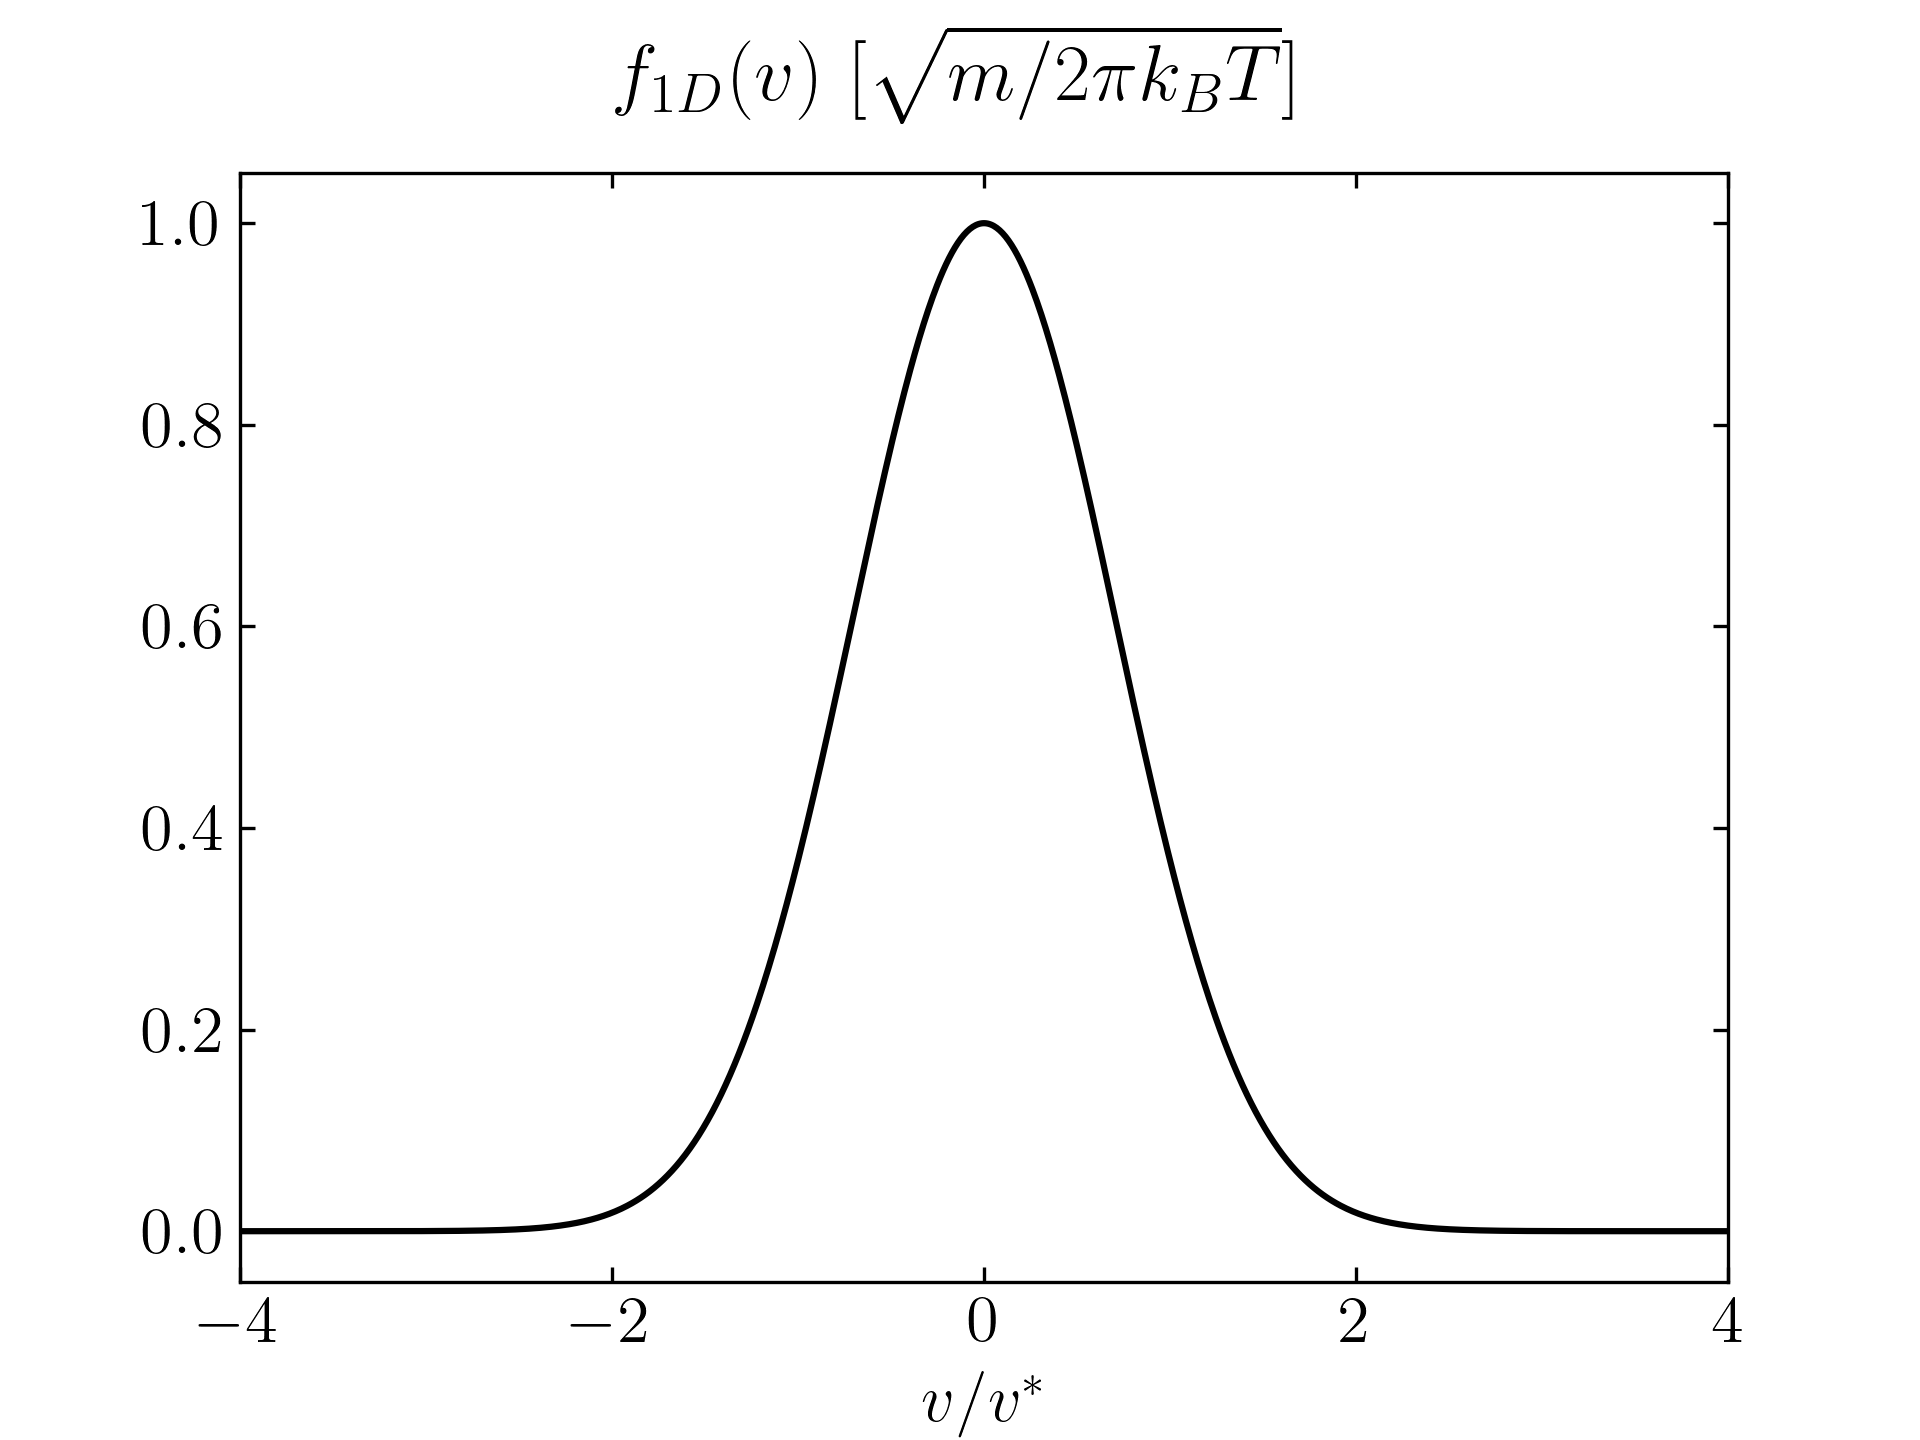
\includegraphics[width=0.8\textwidth]{p5a.png} 
\end{center}

\end{solution}


(b) What is the closely related Maxwell's probability distribution
of \textit{speed} in such a Boltzmann gas

\begin{solution}
 The speed
distribution function is obtained by integrating over the solid angle $d\Omega$,
leaving
\begin{equation}
    f(v)dv
    =\int v^2d\Omega dv f_{3D}(\vb{v}_i)
    =4\pi v^2\qty(\frac{m}{2\pi k_BT})^{3/2}e^{-\beta(1/2)mv^2}dv.
\end{equation}
A plot of $f(v)$ is given below.
\begin{center}
    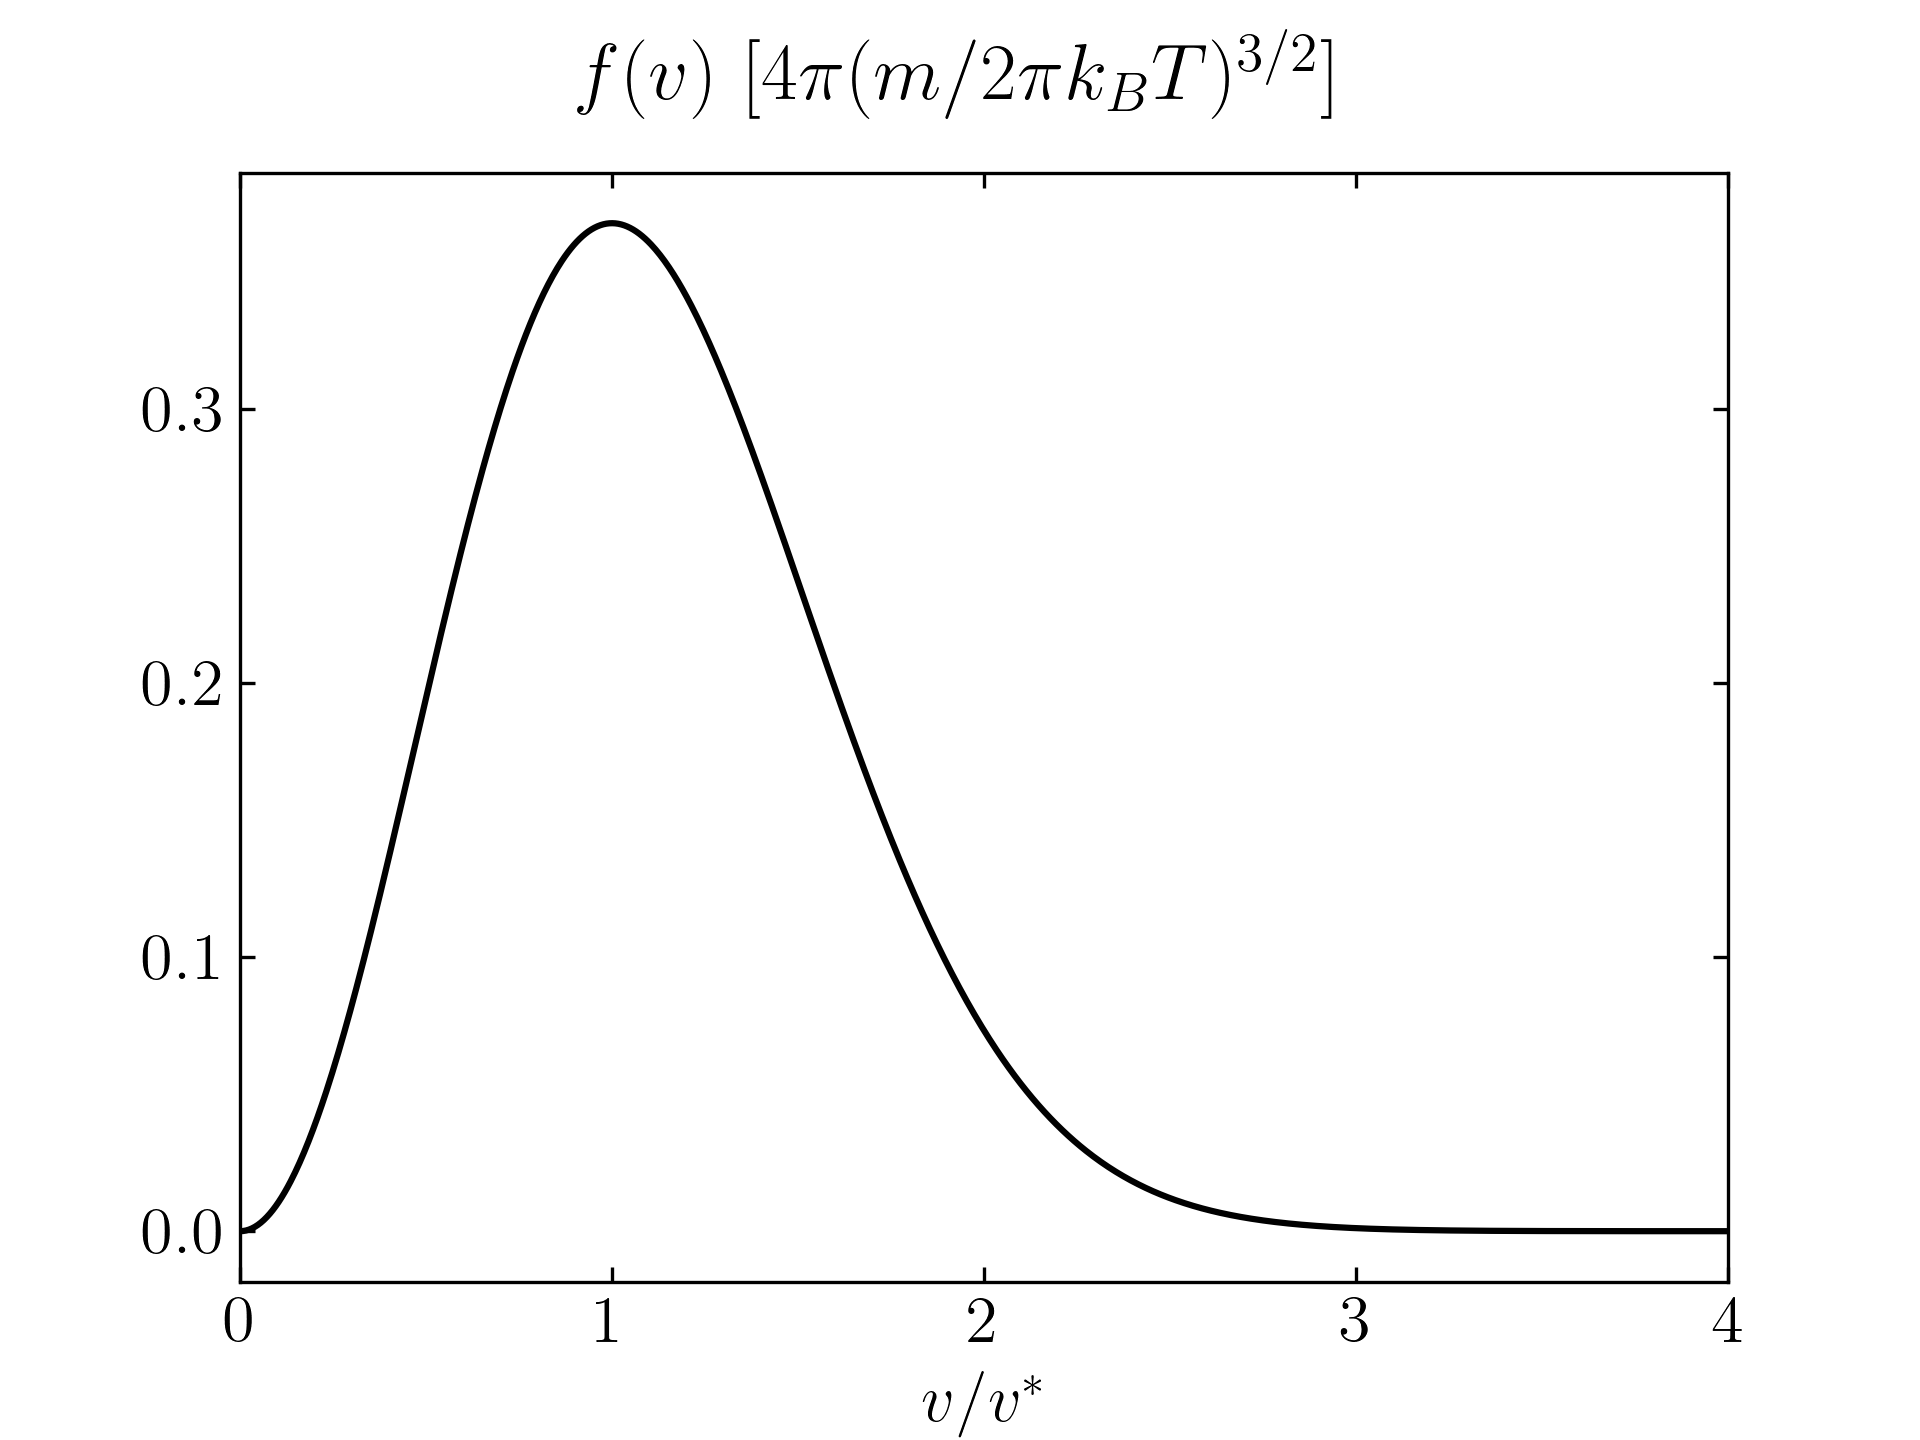
\includegraphics[width=0.8\textwidth]{p5b.png} 
\end{center}
\end{solution}

(c) Identify the width of the velocity distribution, $v_{rms}$, and estimate
from it and the figure in (b) of the typical speed of an oxygen molecule in
room-temperature air.
\begin{solution}
By definition,

\begin{align}
    v_{rms}
    &=\sqrt{\expval{v^2}}\notag\\
    &=\sqrt{\int dv v^2f(v)}\notag\\
    &=\sqrt{4\pi\qty(\frac{m}{2\pi
    k_BT})^{3/2}3\sqrt{\frac\pi2}\qty(\frac{k_BT}{m})^{5/2}}\notag\\
    &=\sqrt{\frac{3k_BT}{m}}.
\end{align}
Let the room temperature be $T=300$\,\si{K}. Given that the mass of one oxygen 
molecule is $m_{O_2}=5.3\times10^{-26}$\,\unit{kg}, we can calculate the rms 
speed to be $v_{rms}\approx484$\,\si{m/s}. The mean speed for a Maxwellian is
$\expval{v}=\sqrt{2k_BT/m}=395$\,\si{m/s}. Thus, an oxygen molecule typically
has a speed in the range from 89\,\si{m/s} to 879\,\si{m/s}.
\end{solution}

(d) By integrating over $6N$ dimensional phase space and using the Gaussian
integrals calculus above, compute the partition function
\begin{equation}
    Z(T)=\frac1{N!}\prod_{i=1}^N\qty[\int\frac{d\vb{r}_id\vb{p}_i}{(2\pi\hbar)^3}]e^{-\beta\HH}
    ,
\end{equation}
where $1/N!$ is the Gibbs ``fudge'' factor to crudely (we will see later why
this fix fails at low temperatures; also see below) account for the identity of
these classical particles, and we use the fact that 1 state corresponds to phase
space are $dxdp=2\pi\hbar$ to normalize the integration measure.

Note: Compare to your result in microcanonical ensemble and marvel at simplicity
of the computation in the canonical ensemble.

\begin{solution}
Given the definition, we carry out the computation
\begin{align}
    Z(T)
    &\approx\frac{V^N}{e^{-N}N^N}\frac1{h^{3N}}\prod_{i=1}^N\int d^3\vb{p}_i
    e^{-\beta \vb{p}_i^2/2m}\notag\\
    &=\frac{V^N}{e^{-N}{N^N}}
    \frac1{h^{3N}}\qty(\int_{-\infty}^\infty dp_ie^{-\beta
    p_i^2/2m})^{3N}\notag\\
    &=\frac{V^N}{e^{-N}N^N}\frac1{h^{3N}}\qty(\sqrt{\frac{2\pi}{\beta/m}})^{3N}\notag\\
    &=\frac{V^N}{e^{-N}N^N}\qty(\frac{\sqrt{2\pi mk_BT}}{h})^{3N}\notag\\
    &=\frac{e^N}{\qty(n\lambda_{dB}^3)^N},
\end{align}
where $\lambda_{dB}(T)$ is the deBroglie wavelength.
\end{solution}

(e) Compute the corresponding (i) free energy $F(T)$, (ii) entropy $S(T)$, and
(iii) the average energy $E(T)$.

\begin{solution}

(i) From (d), the free energy is
\begin{equation}
    F=-Nk_BT\ln\qty(\frac{e}{n\lambda_{dB}^3})
    =Nk_BT\qty[\ln\qty(n\lambda_{dB})-1].
\end{equation}

(ii) Then, the entropy is (using Mathematica)
\begin{equation}
    S=-\frac{\partial F}{\partial T}
    =Nk_B\qty[\frac52-\ln\qty(n\lambda_{dB}^3)].
\end{equation}

(iii) And the average energy (again, with Mathematica) is
\begin{equation}
    E=F+TS
    =\frac32Nk_BT.
\end{equation}
\end{solution}

(f) Using the expression for $F(T,V,N)$ found above, calculate the pressure
$P(T,V,N)$ for the Boltzmann gas, and show that it leads to the familiar ideal
gas law, $PV=Nk_BT$.

\begin{solution}
As derived in Problem 1c, the pressure is
\begin{equation}
    P=-\frac{\partial F}{\partial V}   
    =-Nk_BT\frac{\partial}{\partial V}\qty[\ln\qty(\frac{N\lambda_{dB}^3}{V})]
    =\frac{Nk_BT}{V}\Rightarrow PV=Nk_BT
\end{equation}
\end{solution}

(g) Compute the corresponding chemical potential, expressing it in terms of
thermal deBroglie wavelength, and density $n$.

\begin{solution}
Similarly,
\begin{equation}
    \mu=\frac{\partial F}{\partial N}
    =k_BT\frac{\partial}{\partial N}\qty[N\ln\qty(\frac{N\lambda_{dB}^3}{V})-1]
    =k_BT\ln\qty(n\lambda_{dB}^3)
\end{equation}
This is exactly the same as HW1's result.
\end{solution}

\end{problem}
\newpage
%%%%%%%%%%%%%%%%%%%%%%%%%%%%%%%%%%%%%%%%%%%%%%%%%%%%%%%%%%%%%%%%%%%%%%%%%%%%%%%
%%%%%%%%%%%%%%%%%%%%%%%%%%%%%%%%%%%%%%%%%%%%%%%%%%%%%%%%%%%%%%%%%%%%%%%%%%%%%%%
\begin{problem}{6}[Classical harmonic oscillators: Einstein solid]
Let's now re-examine $N$ decoupled 3D classical harmonic oscillators, described
by the familiar Hamiltonian
\begin{equation}
    \HH=\sum_{i=1}^N\qty[\frac{\vb{p}_i^2}{2m}+\frac12m\omega_0^2\vb{r}_i^2] ,
\end{equation}
as the classical version of the problem above, with $\vb{r}_i,\vb{p}_i$ the
classical phase-space coordinates. Let's repeat the analysis utilizing and
generalizing the analysis for the Boltzmann gas, above.

(a) By integrating over $6N$ dimensional phase-space, compute the partition
function
\begin{equation}
   Z(T)=\prod_{i=1}^N\qty[\int\frac{d\vb{r}_id\vb{p}_i}{(2\pi\hbar)^3}]e^{-\beta\HH} 
\end{equation}
where there is no $1/N!$ Gibbs ``fudge'' factor, as discussed before.
\begin{solution}
By definition,
\begin{align}
    Z(T)
    &=\frac1{(2\pi\hbar)^{3N}}\prod_{i=1}^N\int d\vb{r}_id\vb{p}_i
    \exp\qty(-\beta\frac{\vb{p}_i^2}{2m}-\frac12\beta
    m\omega_0^2\vb{r}_i^2)\notag\\
    &=\frac1{(2\pi\hbar)^{3N}}\qty(\int_{-\infty}^\infty dr_ie^{-(1/2)\beta
    m\omega_0^2r_i^2}\int_{-\infty}^\infty dp_ie^{-\beta p_i^2/2m})^{3N}\notag\\
    &=\frac1{(2\pi\hbar)^{3N}}\qty(\sqrt{\frac{2\pi}{\beta
    m\omega_0^2}}\sqrt{\frac{2\pi}{\beta/m}})^{3N}\notag\\
    &=\qty(\frac{k_BT}{\hbar\omega_0})^{3N}
\end{align}
\end{solution}

(b) Compare your classical result with the high $T$ classical limit
($\hbar\omega_0/k_BT$ is the relevant dimensionless parameter) of the quantum
treatment of the system in problem 4(d), above.
\begin{solution}
    This is the same as \eqref{p4d:Z}. There's nothing else to compare.
\end{solution}

(c) Using the observation that $\Omega(E)$ is an inverse Laplace transform of
$Z(\beta)$, use above result for $Z(\beta)$ of $N$ classical harmonic
oscillators to obtain the corresponding $\Omega(E)$ that you found in the
microcanonical ensemble in previous homeork set.
\begin{solution}
    Given that $Z(\beta)=\LL\qty(\Omega(E)/\Delta)$ where $\LL$ is the Laplace
    transform, then
    \begin{equation}
        \Omega(E)=\Delta\LL^{-1}\qty[F(\beta)] 
        =\frac{\Delta}{(\hbar\omega_0)^{3N}}\LL^{-1}\qty[\frac1{\beta^{3N}}]
    \end{equation}
    Plugging this into Mathematica, we get
    \begin{equation}
        \Omega(E)=\frac{\Delta}{E}\qty(\frac{E}{\hbar\omega_0})^{3N}\frac1{\Gamma(3N)}
        \approx\frac{\Delta}{E}\qty(\frac{E}{3N\hbar\omega_0})^{3N},
    \end{equation}
    which is the same result from the microcanonical ensemble approach.
\end{solution}
\end{problem}
\newpage
%%%%%%%%%%%%%%%%%%%%%%%%%%%%%%%%%%%%%%%%%%%%%%%%%%%%%%%%%%%%%%%%%%%%%%%%%%%%%%%

%%%%%%%%%%%%%%%%%%%%%%%%%%%%%%%%%%%%%%%%%%%%%%%%%%%%%%%%%%%%%%%%%%%%%%%%%%%%%%%
\begin{problem}{7}[Partition function of a classical string under tension]
In lecture and above we studied independent harmonic oscillators. Let's now
consider statistical mechanics of \textit{coupled} classical harmonic
oscillators, which physically can come in a form of any elastic medium (e.g., a
membrane), here focusing on an elastic string under tension. Such a problem is
in fact of relevance and has been studied extensively in a context of polymer
elasticity, e.g., pulling on a DNA with optical tweezers [see Marko and Siggia,
Macromolecules 1995, 28, 8759-8770], as is done experimentally by our colleague
Tom Perkins in JILA (see Fig. 1). It is also of relevance to the study of
entropic (thermal) elasticity of rubber.

n principle a microscopic model of a polymer is that of $N$ atoms connected by 
chemical bonds, that can be modeled by harmonic springs and with ends fixed. 
However, below we will simplify this description by a continuum Hamiltonian, 
only adding atomic “granuality” after the fact by putting a cutoff on normal 
modes set by the atomic spacing $a$. Also for simplicity we will use periodic 
(rather than fixed ends) boundary conditions.

The appropriate continuum Hamiltonian is given by,
\begin{equation}
    \HH=\frac\sigma2\int_0^Ldx\qty(\partial h/\partial x)^2,
\end{equation}
where $\sigma$ is the elastic stretching constant -- polymer's energy per unit
length, and I only included the elastic energy, neglecting kinetic energy, 
which (as we saw above) classically always decouples to the same 
multiplicative contribution to $Z$. $h(x)$ is the transverse (up-down) 
deviation (that for simplicity we take to be a scalar, though in
reality it is a two-dimensional vector) of the polymer from its perfect 
stretched state, $h(x) = 0$, as illustrated in Fig.2.
We note that elastic energy is just a continuum approximation
$(\partial h/\partial x)^2 \approx [h(x + \epsilon -h(x)]^2/\epsilon^2 =
(h_{x_2} -h_{x_1})^2$ neighboring displacements $h(x_1)$ and $h(x_2)$ coupled 
by a harmonic spring. We can decouple these by going from coupled $h(x)$ 
degrees of reedom to decoupled normal modes. Translational invariance 
guarantees that this can be implemented via Fourier series transform with the 
normal modes just the Fourier mode amplitudes, $\tilde{h}_k$,
\begin{equation}\label{p7:Fh}
    h(x)=\frac1{\sqrt{L}}\sum_k\tilde{h}_ke^{ikx}, 
\end{equation}
where simplifying periodic boundary conditions require $k_n=2\pi n/L$ to be
discrete.

(a) Using this Fourier transform representation \eqref{p7:Fh} inside the string
elastic Hamiltonian, express $\HH\qty[h(x)]$ in terms of $\tilde{h}_k$ and give
the resulting $\HH[\qty{h_k}]$. \textit{Hint}: Use the standard orthogonality
of harmonic functions in integrating over $x$.
\begin{solution}
Given $h(x)$ in \eqref{p7:Fh}, we can calculate
\begin{equation}
    \frac{\partial h}{\partial
    x}=\frac{i}{\sqrt{L}}\sum_{k}k\tilde{h}_ke^{ikx}, 
    =\frac{i}{\sqrt{L}}\sum_{n=-N}^N\frac{2\pi n}{L}\tilde{h}_k(n)e^{i2\pi
    nx/L}.
\end{equation}
Then, the Hamiltonian is
\begin{align}
    \HH
    &=-\frac{\sigma}{2L}\int_0^Ldx\qty(\sum_{n=-N}^N\frac{2\pi
    n}{L}\tilde{h}_k(n)e^{i2\pi nx/L})^2\notag\\
    &=\sigma\sum_{n=1}^N\qty(\frac{2\pi
    n}{L})^2\tilde{h}_k(-n)\tilde{h}_k(n)
\end{align}
\end{solution}

(b) Noting that $\tilde{h}_k=h_{Rk}+ih_{Ik}$ are complex (as Fourier
coefficients generically are), show from \eqref{p7:Fh} that they are not
independent and satisfy $\tilde{h}_{-k}=\tilde{h}_{k}^\ast$ where ``star'' is
complex conjugation.
\begin{solution}
By definition, the Fourier amplitudes are determined as
\begin{equation}\label{p7b:hk}
    \tilde{h}_k=\int dxh(x)e^{-ikx}
    =\int dxh(x)\cos\qty(kx)-i\int dxh(x)\sin\qty(kx).
\end{equation}
Now, under a parity flip,
\begin{equation}
    \tilde{h}_{-k}=\int dxh(x)\cos(kx)+i\int dxh(x)\sin(kx)
    =\tilde{h}_k^\ast.
\end{equation}
Thus, the Fourier coefficients are not independent, and in fact, they follow the
symmetry $\tilde{h}_k=\tilde{h}_{-k}^\ast$ as shown.
\end{solution}

(c) Note that in the $k$ summation (e.g., inside $\HH$), we sum over both
positive and negative $k$'s, with non-independent $\tilde{h}_k$'s. Show that
using previous condition (b), you can reduce the sum to only positive $k$ of
fully \textit{independent real} numbers $h_{Rk}$ and $h_{Ik}$, that
characterizes the microstates of the fluctuating string.

Show, thereby that this accomplishes the desired result of reducing $\HH$ to a
sum of independent harmonic oscillators, $\qty{h_{Rk},h_{Ik}}$, two per each
positive mode $k$, and write down explicitly and in all detail the resulting
$\HH\qty[\qty{h_{Rk},h_{Ik}}]$.
\begin{solution}
From \eqref{p7:Fh}, we can write
\begin{align}
h(x)
&=\frac1{\sqrt{L}}\qty[\sum_{k<0}\tilde{h}_ke^{ikx}+\tilde{h}_0+\sum_{k>0}\tilde{h}_ke^{ikx}]\notag\\
&=\frac1{\sqrt{L}}\qty[
\tilde{h}_0+\sum_{k>0}\qty(\tilde{h}_{-k}e^{-ikx}+\tilde{h}_ke^{ikx})
]\notag\\
&=\frac1{\sqrt{L}}
\qty[
\tilde{h}_0
+2\sum_{k>0}\qty(h_{Rk}\cos(kx)-h_{Ik}\sin\qty(kx))
],
\end{align}
where $h_{Rk},h_{Ik}$ are components of \eqref{p7b:hk}. This expression is
reduced to only positive $k$ of fully independent real numbers, as desired.

From part (a), we can then write
\begin{equation}
    \HH=\sigma\sum_{n=1}^N\qty(\frac{2\pi n}{L})^2\abs{\tilde{h}_k(n)}^2
    =\sigma\sum_{n=1}^N\qty(\frac{2\pi n}{L})^2\qty(h_{Rk}^2+h_{Ik}^2)
    =\sigma\sum_{k>0}k^2\qty(h_{Rk}^2+h_{Ik}^2)
\end{equation}
\end{solution}

(d) What is the effective stiffness $J_k$ (which determines the natural
frequency $\omega_k$ with $J_k=\omega_k^2$) of a normal mode $k$, reading it off
from your result in (c) above.

\begin{solution}
Since $\qty[\tilde{h}_k]=m^{3/2}$, the stiffness should be
$J_k=\omega_k^2=\sigma(2\pi n)^2/L$. 
\end{solution}

(e) Now we can straightforwardly utilize our expertise about classical decoupled
harmonic oscillators to compute all of thermodynamics

\qquad(i) Compute the (i) partition function, $Z$ and the (ii) associated free
energy $F$.
\begin{solution}
By definition,
\begin{align}
Z&=\int\frac{dh_{Rk}dh_{Ik}}{\lambda_T^3}\exp\qty[-\beta\sigma\sum_{k>0}k^2(h_{Rk}^2+h_{Ik}^2)]\notag\\
 &=\frac1{\lambda_T^{3N}}\qty[\int dh e^{-\beta\sigma k^2h^2}]^{2N}\notag\\
 &=\frac1{\lambda_T^{3N}}\qty(\sqrt{\frac{2\pi}{2\beta\sigma k^2}})^{2N}\notag\\
 &=\qty(\frac{\pi k_BT}{\sigma\lambda_T(k\lambda_T)^2})^N
\end{align}
where $N$ is the number of positive $k$ states, $\lambda_T$ is the deBroglie
wavelength. The energy then follows
\begin{equation}
    F=Nk_BT\ln\qty(\frac{\sigma\lambda_T(k\lambda_T)^2}{\pi k_BT})
\end{equation}

\textit{Note}: Not sure if this is even the correct answer... I've been working
non-stop for 36 hours. So I think I'm giving up here :)

\end{solution}


\end{problem}
\newpage
%%%%%%%%%%%%%%%%%%%%%%%%%%%%%%%%%%%%%%%%%%%%%%%%%%%%%%%%%%%%%%%%%%%%%%%%%%%%%%%
    
\end{document}
